%%%%%%%%%%%%%%%%%%%%%%%%%%%%%%%%%%%%%%%%%%%%%%%%%%%%%%%%%%%%%%%%%%%%%%
% njuthesis 示例模板 v1.4.3 2025-05-21
% https://github.com/nju-lug/NJUThesis
%
% 贡献者
% Yu XIONG @atxy-blip   Yichen ZHAO @FengChendian
% Song GAO @myandeg     Chang MA @glatavento
% Yilun SUN @HermitSun  Yinfeng LIN @linyinfeng
% Yukai Chou @Muzimuzhi
%
% 许可证
% LaTeX Project Public License（版本 1.3c 或更高）
%%%%%%%%%%%%%%%%%%%%%%%%%%%%%%%%%%%%%%%%%%%%%%%%%%%%%%%%%%%%%%%%%%%%%%

%---------------------------------------------------------------------
% 一些提升使用体验的小技巧：
%   1. 请务必使用 UTF-8 编码编写和保存本文档
%   2. 请务必使用 XeLaTeX 或 LuaLaTeX 引擎进行编译
%   3. 不保证接口稳定，写作前一定要留意版本号
%   4. 以百分号(%)开头的内容为注释，可以随意删除
%---------------------------------------------------------------------

%---------------------------------------------------------------------
% 请先阅读使用手册：
% http://mirrors.ctan.org/macros/unicodetex/latex/njuthesis/njuthesis.pdf
%---------------------------------------------------------------------

\documentclass[
    % 模板选项(注意右端逗号)：
    %
    % type = bachelor|master|doctor|postdoc, % 文档类型，默认为本科生
    % degree = academic|professional,        % 学位类型，默认为学术型
    %
    % nl-cover,   % 是否需要国家图书馆封面，默认关闭
    % decl-page,  % 是否需要诚信承诺书或原创性声明，默认关闭
    %
    %   页面模式，详见手册说明
    % draft,                  % 开启草稿模式
    % anonymous,              % 开启盲审模式
    % minimal,                % 开启最小化模式
    %
    %   单双面模式，默认为适合印刷的双面模式
    % oneside,                % 单面模式，无空白页
    % twoside,                % 双面模式，每一章从奇数页开始
    %
    %   字体设置，不填写则自动调用系统预装字体，详见手册
    fontset = fandol, % 使用 TeX Live 自带字体，跨平台更容易直接编译
  ]{njuthesis}

% 模板选项设置，包括个人信息、外观样式等
% 较为冗长且一般不需要反复修改，我们把它放在单独的文件里
\input{docs/njuthesis-setup.def}

% 自行载入所需宏包
% \usepackage{subcaption} % 嵌套小幅图像，比 subfig 和 subfigure 更新更好
% \usepackage{siunitx} % 标准单位符号
% \usepackage{physics} % 物理百宝箱
% \usepackage[version=4]{mhchem} % 绘制分子式
% \usepackage{listings} % 展示代码
% \usepackage{algorithm,algorithmic} % 展示算法伪代码
\usepackage{booktabs}
\usepackage{multirow}
\usepackage{makecell}
\graphicspath{{docs/}}

% 在导言区随意定制所需命令
% \DeclareMathOperator{\spn}{span}
% \NewDocumentCommand\mathbi{m}{\textbf{\em #1}}

% 开始编写论文
\begin{document}

%---------------------------------------------------------------------
%	封面、摘要、前言和目录
%---------------------------------------------------------------------

% 生成封面页
\maketitle

% 模板默认使用 \flushbottom，即底部平齐
% 效果更好，但可能出现 underfull \vbox 信息
% 以下命令用于抑制这些信息
\raggedbottom

\begin{abstract}
  乙型肝炎病毒（HBV）形成感染性颗粒时，成熟核衣壳需要被包膜蛋白识别。本文以HBV核心蛋白HBc和表面蛋白HBsAg preS区为研究对象，选取preS 87--114片段进行体外分析。实验未使用感染性病毒，而是用重组蛋白建立HBc--preS检测流程，并比较preS突变体和候选小分子处理后的信号变化。高浓度Triton X-100和香叶醇处理后，HBc--preS相关读数下降；preS R102A、H105A和W111A突变也减弱结合信号。结果支持preS 87--114参与HBc识别，可作为后续分析HBV包膜化界面和筛选相关抗病毒候选分子的体外依据。
\end{abstract}

\begin{abstract*}
  During the formation of infectious hepatitis B virus (HBV) particles, mature nucleocapsids need to be recognized by envelope proteins. This study focused on HBV core protein (HBc) and the preS region of hepatitis B surface antigen (HBsAg), and selected the preS 87--114 fragment for in vitro analysis. No infectious virus was used. Instead, recombinant proteins were used to establish HBc--preS detection workflows and to compare signal changes after treatment with preS mutants and candidate small molecules. After treatment with high concentrations of Triton X-100 and geraniol, HBc--preS-related readouts decreased; the preS R102A, H105A, and W111A mutations also reduced binding signals. These results support the involvement of preS 87--114 in HBc recognition and provide an in vitro basis for further analysis of the HBV envelopment interface and screening of related antiviral candidate molecules.
\end{abstract*}

% 生成目录
\tableofcontents
% 生成图片清单
% \listoffigures
% 生成表格清单
% \listoftables

%---------------------------------------------------------------------
%	正文部分
%---------------------------------------------------------------------
\mainmatter

% 符号表
% 语法与 description 环境一致
% 两个可选参数依次为说明区域宽度、符号区域宽度
% 带星号的符号表(notation*)不会插入目录
% \begin{notation}[10cm]
%   \item[DFT] 密度泛函理论 (Density functional theory)
%   \item[DMRG] 密度矩阵重正化群 (Density-Matrix Reformation-Group)
% \end{notation}

% 建议将论文内容拆分为多个文件
% 即新建一个 chapters 文件夹
% 把每一章的内容单独放入一个 .tex 文件
% 然后在这里用 \include 导入，例如
%   \include{chapters/introduction}
%   \include{chapters/environments}
% 本示例已经按章节拆分，可直接在 docs/chapters/ 中继续写作
\chapter{绪论}

\section{乙型肝炎病毒感染、生命周期与抗病毒治疗需求}

乙型肝炎病毒（hepatitis B virus, HBV）感染是全球范围内最重要的慢性病毒感染之一，也是肝硬化和肝细胞癌（hepatocellular carcinoma, HCC）的主要病因之一。HBV感染既可表现为急性自限性肝炎，也可发展为长期持续的慢性感染；后者在长期炎症、肝细胞损伤与再生、病毒蛋白表达及宿主免疫压力共同作用下，可显著增加终末期肝病和肝癌风险\cite{dusheiko2023new,lin2020association}。虽然预防性疫苗已经显著降低了新发感染率，核苷（酸）类似物和干扰素治疗也能够有效抑制病毒复制，但现有治疗通常难以彻底清除感染细胞内的共价闭合环状DNA（cccDNA）及相关病毒遗传物质。因此，慢性HBV感染仍常需要长期治疗和随访，停药后病毒学反弹、药物耐受性以及残余肝癌风险等问题依然存在。

从药物开发角度看，HBV生命周期中的多个步骤均可能成为抗病毒干预靶点。传统核苷（酸）类似物主要抑制病毒聚合酶介导的逆转录过程，而近年来针对病毒进入、衣壳组装、cccDNA维持、病毒RNA稳定性以及宿主免疫调节等环节的策略也受到关注\cite{selzer2015assembly,taverniti2022capsid}。其中，感染性病毒颗粒的形成依赖于病毒核衣壳与包膜蛋白之间的特异性识别和装配。该过程位于病毒复制后期，直接决定成熟核衣壳能否被包膜包裹并分泌为具有感染性的Dane颗粒。若能够选择性阻断核衣壳包膜化，理论上可在不完全依赖聚合酶抑制的情况下减少感染性病毒颗粒释放，从而为开发新型抗HBV药物提供补充方向。

在这一背景下，理解HBV感染性颗粒形成的分子机制，对于寻找区别于传统聚合酶抑制的新型干预策略具有重要意义。HBV是一种有包膜的小型DNA病毒，病毒颗粒内部为由核心蛋白（hepatitis B core protein, HBc）组装而成的二十面体核衣壳，外部包裹含有乙肝表面抗原（hepatitis B surface antigen, HBsAg）的脂质膜\cite{venkatakrishnan2016structural}。HBc蛋白可通过二聚体作为基本单元自发组装成T=3或T=4对称性的核衣壳，其中T=4颗粒在体外和病毒颗粒中均较为常见。核衣壳不仅为前基因组RNA（pgRNA）和病毒聚合酶提供封装空间，也为逆转录反应提供受限的内部环境。随着pgRNA逆转录为松弛环状DNA，核衣壳逐渐成熟，并获得参与后续包膜化和分泌的能力。

HBV感染性颗粒的形成并不是核衣壳随机被细胞膜包裹的过程，而是一个需要病毒蛋白之间精确匹配的形态发生事件。成熟核衣壳需在内质网及其相关膜系统附近与HBsAg发生相互作用，随后通过细胞分泌途径释放\cite{bruss2007morphogenesis,selzer2015assembly}。这一过程具有高度选择性：一方面，未成熟核衣壳一般不能高效进入分泌途径；另一方面，HBsAg本身可以大量形成不含核衣壳的亚病毒颗粒（subviral particles, SVPs），说明表面蛋白外排与感染性病毒颗粒包膜化虽然共享部分膜运输路径，却并非完全相同的机制。因而，核衣壳与包膜蛋白之间的特异性相互作用被认为是HBV形态发生的核心调控节点。

\section{HBsAg preS区域在核衣壳包膜化中的功能}

HBsAg由同一开放阅读框通过不同翻译起始位点产生三种相关蛋白：小表面蛋白S-HBsAg、中表面蛋白M-HBsAg和大表面蛋白L-HBsAg\cite{seitz2020envelope}。三者共享S结构域；M-HBsAg在N端额外含有preS2区域；L-HBsAg进一步包含preS1和preS2区域，二者合称preS区域。遗传学研究显示，L-HBsAg和S-HBsAg对于感染性病毒颗粒的形成不可或缺，而M-HBsAg在许多实验体系中并非病毒颗粒分泌的必需组分\cite{bruss1991role,ni2010pres2}。这一现象提示，L-HBsAg特有的preS区域在病毒颗粒成熟过程中承担了特殊功能。

L-HBsAg的一个重要特征是preS区域具有双重跨膜拓扑。部分preS位于病毒颗粒外侧，能够在感染早期介导病毒与肝细胞受体NTCP结合，并参与后续入侵过程\cite{yan2012ntcp,asami2024structural}；另一部分preS则朝向病毒颗粒内侧或细胞质侧，被认为参与核衣壳包膜化。强制改变L-HBsAg拓扑、使preS仅呈外向型分布，会阻断病毒颗粒分泌而不明显影响核衣壳装配，说明内向型preS与核衣壳的接触是病毒形态发生所需的独立步骤\cite{bruss1995functions,seitz2020envelope}。因此，preS区域同时连接了HBV入侵和组装两个关键阶段，是病毒生命周期中的多功能调控区。

preS区域还具有重要的临床和病理学意义。慢性HBV感染患者中可出现自然发生的preS缺失或突变，这些变异与表面蛋白滞留、内质网应激、免疫逃逸、病毒颗粒分泌异常以及HCC发生风险升高有关\cite{lin2020association,peiffer2018divergent}。从机制角度看，preS突变不仅可能影响受体结合和抗原性，也可能改变L-HBsAg与核衣壳的相互作用，进而影响病毒颗粒形成效率和病毒群体组成。因此，解析preS如何识别HBc，不仅有助于理解HBV形态发生，也有助于解释慢性感染过程中某些preS变异被选择和维持的原因。

围绕preS功能的早期遗传学和生化研究已经证明，L-HBsAg的preS区域与HBc核衣壳之间存在功能性联系。preS1内部的一段短线性序列被证实对病毒颗粒形成至关重要，相关区域的缺失或突变会显著损害Dane颗粒分泌，但未必影响表面蛋白形成亚病毒颗粒\cite{bruss1995functions,bruss1997short}。Bruss进一步通过linker substitution和双丙氨酸扫描突变，将这一功能区缩小到preS1 C端约27个氨基酸范围内；这些突变体仍可产生相对稳定的L蛋白并与S蛋白共同形成亚病毒颗粒，但部分突变显著削弱感染性病毒颗粒释放\cite{bruss1997short}。根据该研究对preS功能区的定位，preS 87--114可被视为preS与core发生关键相互作用并支持包膜化的核心区域，而不是单纯影响表面蛋白表达或分泌的区域。

\begin{figure}[htbp]
  \centering
  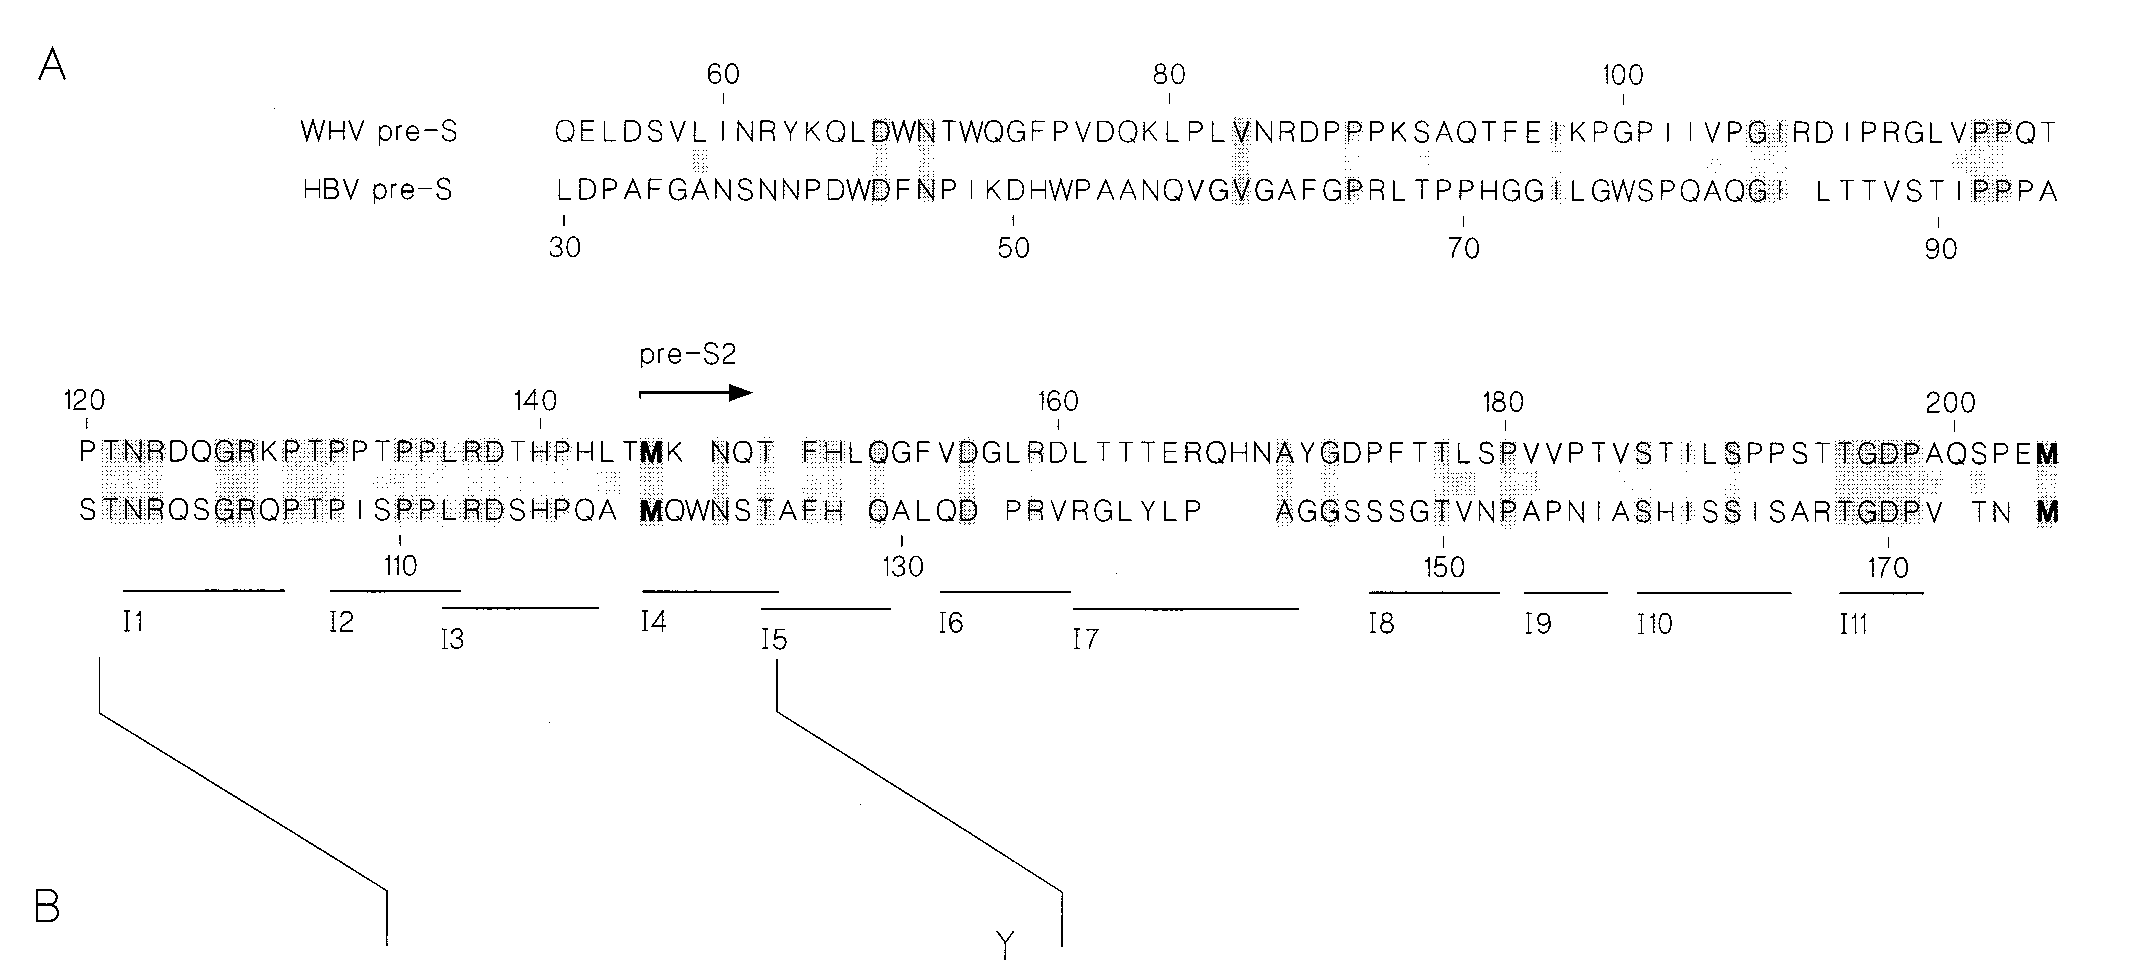
\includegraphics[width=0.86\textwidth]{figures/introduction/bruss1997_pres_mutant_map.png}
  \par\medskip
  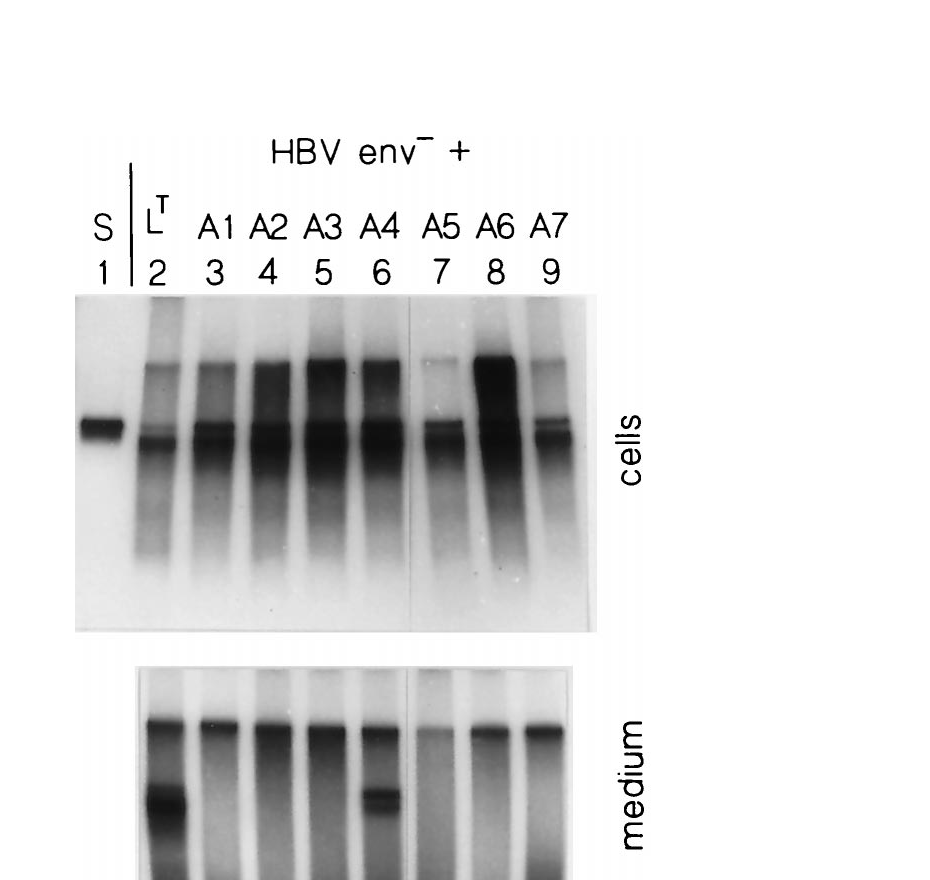
\includegraphics[width=0.42\textwidth]{figures/introduction/bruss1997_virion_complementation.png}
  \caption{preS短线性功能区的早期定位。上图显示Bruss构建的preS突变定位图；下图显示部分双丙氨酸突变体在L蛋白阴性HBV基因组互补实验中的病毒颗粒释放表型。该区域的突变可在保留表面蛋白相关分泌能力的同时削弱病毒颗粒形成，提示其可能参与核衣壳识别和包膜化过程。图片截取自Bruss的研究\cite{bruss1997short}。}
  \label{fig:bruss1997-pres-core-region}
\end{figure}

除preS区域外，S结构域胞质环也被报道具有核心颗粒结合能力。Poisson等利用体外多肽和核心颗粒结合实验发现，preS1相关片段和S区胞质环均可与HBc颗粒发生相互作用\cite{poisson1997both}。后续研究通过ELISA、BIAcore和合成多肽进一步支持了HBV包膜化过程中存在多点接触的模型，认为preS与S区胞质环可能共同稳定核衣壳--包膜复合物\cite{choi2004quantitative,muhamad2015peptide}。然而，这些实验多数依赖短肽、固定化蛋白或体外重构体系，难以完全反映膜环境中全长表面蛋白和核衣壳之间的动态接触。

细胞水平研究也支持L-HBsAg在介导核衣壳--包膜相互作用中的关键作用。共表达实验显示，L-HBsAg能够促进核心蛋白向核周或膜相关区域重新定位，并与核心蛋白发生可检测的共沉淀；相较之下，单独S-HBsAg与核心蛋白之间的相互作用较弱\cite{pastor2019direct}。此外，preS1--preS2衔接区的缺失可破坏核心蛋白重定位和共沉淀，提示该区域对于形成有效的核心蛋白--包膜蛋白复合物十分关键。这些发现将早期多肽研究与细胞内形态发生过程联系起来，进一步强调preS区域是HBV包膜化研究的中心对象。

\section{HBc--preS结合区域与药物靶向潜力}

尽管HBc--preS相互作用已被多种实验证据支持，其高分辨率结构基础长期缺乏。造成这一困难的原因之一在于，单个preS片段与核衣壳的相互作用可能较弱，而真实病毒颗粒中L-HBsAg和HBc二聚体均以多拷贝形式存在，多价效应可能显著增强整体结合稳定性。基于Bruss对preS短线性功能区的定位，preS 87--114被认为是连接L-HBsAg和core的关键区域\cite{bruss1997short}。因此，围绕该区域建立非感染性体外互作检测体系，有助于在较高生物安全性和可控性条件下解析HBc--preS相互作用。

从药物靶向角度看，HBc表面的可结合口袋为干预核衣壳--包膜蛋白相互作用提供了潜在切入点。Makbul等在HBc衣壳样颗粒中观察到Triton X-100（TX100）可结合核心蛋白二聚体界面附近的疏水口袋，ITC测得其与HBc颗粒的结合处于微摩尔量级，并且冷冻电镜密度显示TX100位于由HBc链间残基围成的特定口袋内\cite{makbul2021binding}。该研究说明，HBc表面除经典CAM口袋外还存在能够容纳疏水小分子的局部结构，为后续评价小分子是否影响HBc--preS结合提供了结构线索。

\begin{figure}[htbp]
  \centering
  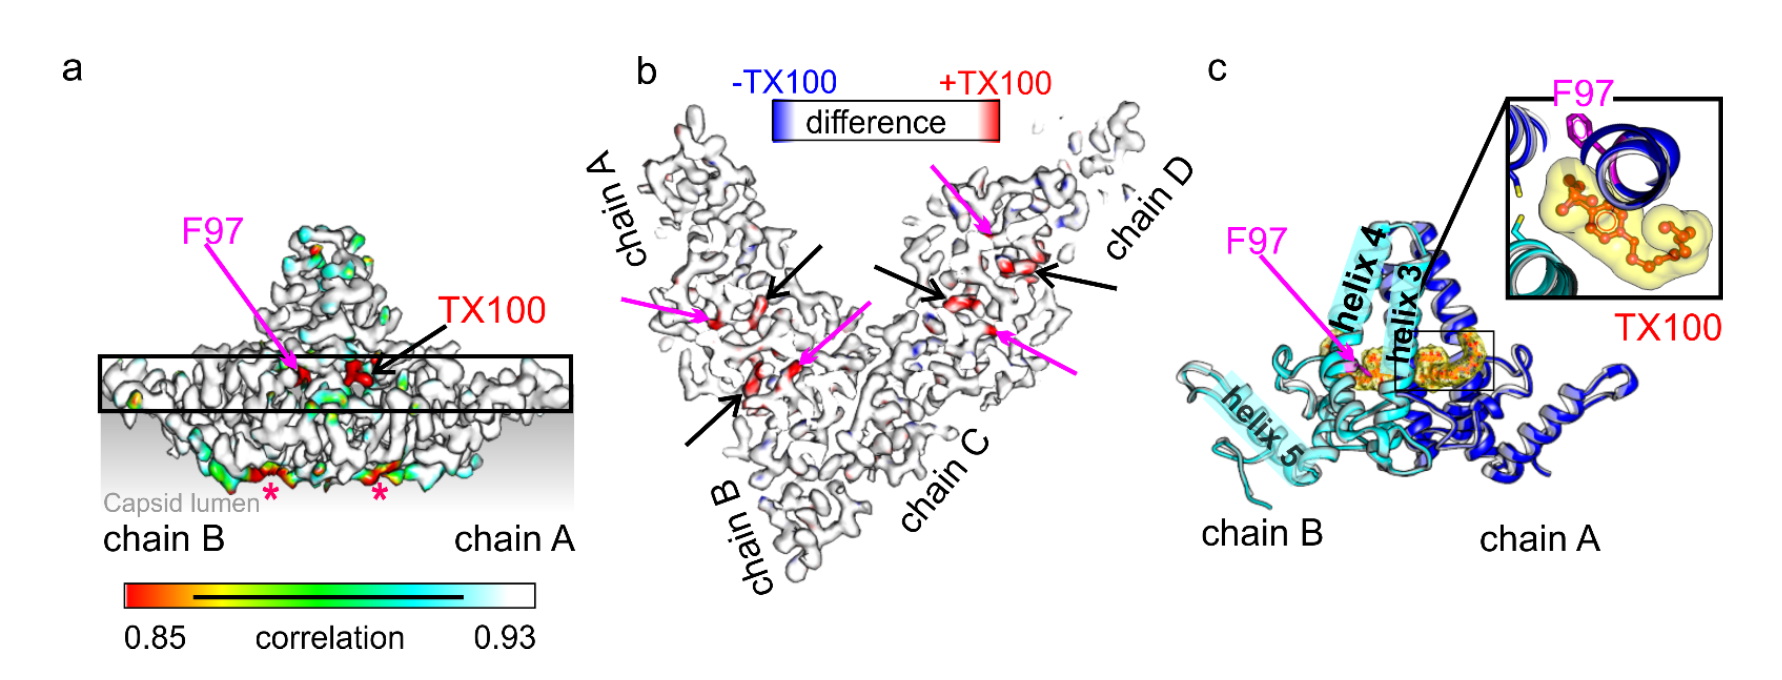
\includegraphics[width=0.70\textwidth]{figures/introduction/makbul2021_tx100_hbc_pocket.png}
  \caption{Triton X-100结合HBc二聚体疏水口袋的结构示意。TX100位于HBc链C和链D形成的二聚体界面附近，并被特定疏水口袋容纳。图片截取自Makbul等的研究\cite{makbul2021binding}。}
  \label{fig:makbul2021-tx100-pocket}
\end{figure}

香叶醇（geraniol）也被报道能够直接结合HBc核心蛋白。Khayenko等结合ITC和冷冻电镜发现，geraniol以微摩尔亲和力结合HBc中心疏水口袋，冷冻电镜图中可在不对称单位内多个疏水口袋观察到geraniol相关密度，并且其结合位置与TX100结合位点发生空间重叠\cite{khayenko2024induction}。因此，TX100和geraniol并不只是非特异性疏水添加剂，而是能够占据HBc特定疏水口袋的小分子。这些已发表研究提示，HBc疏水口袋具有被小分子结合和调控的可能性。

\begin{figure}[htbp]
  \centering
  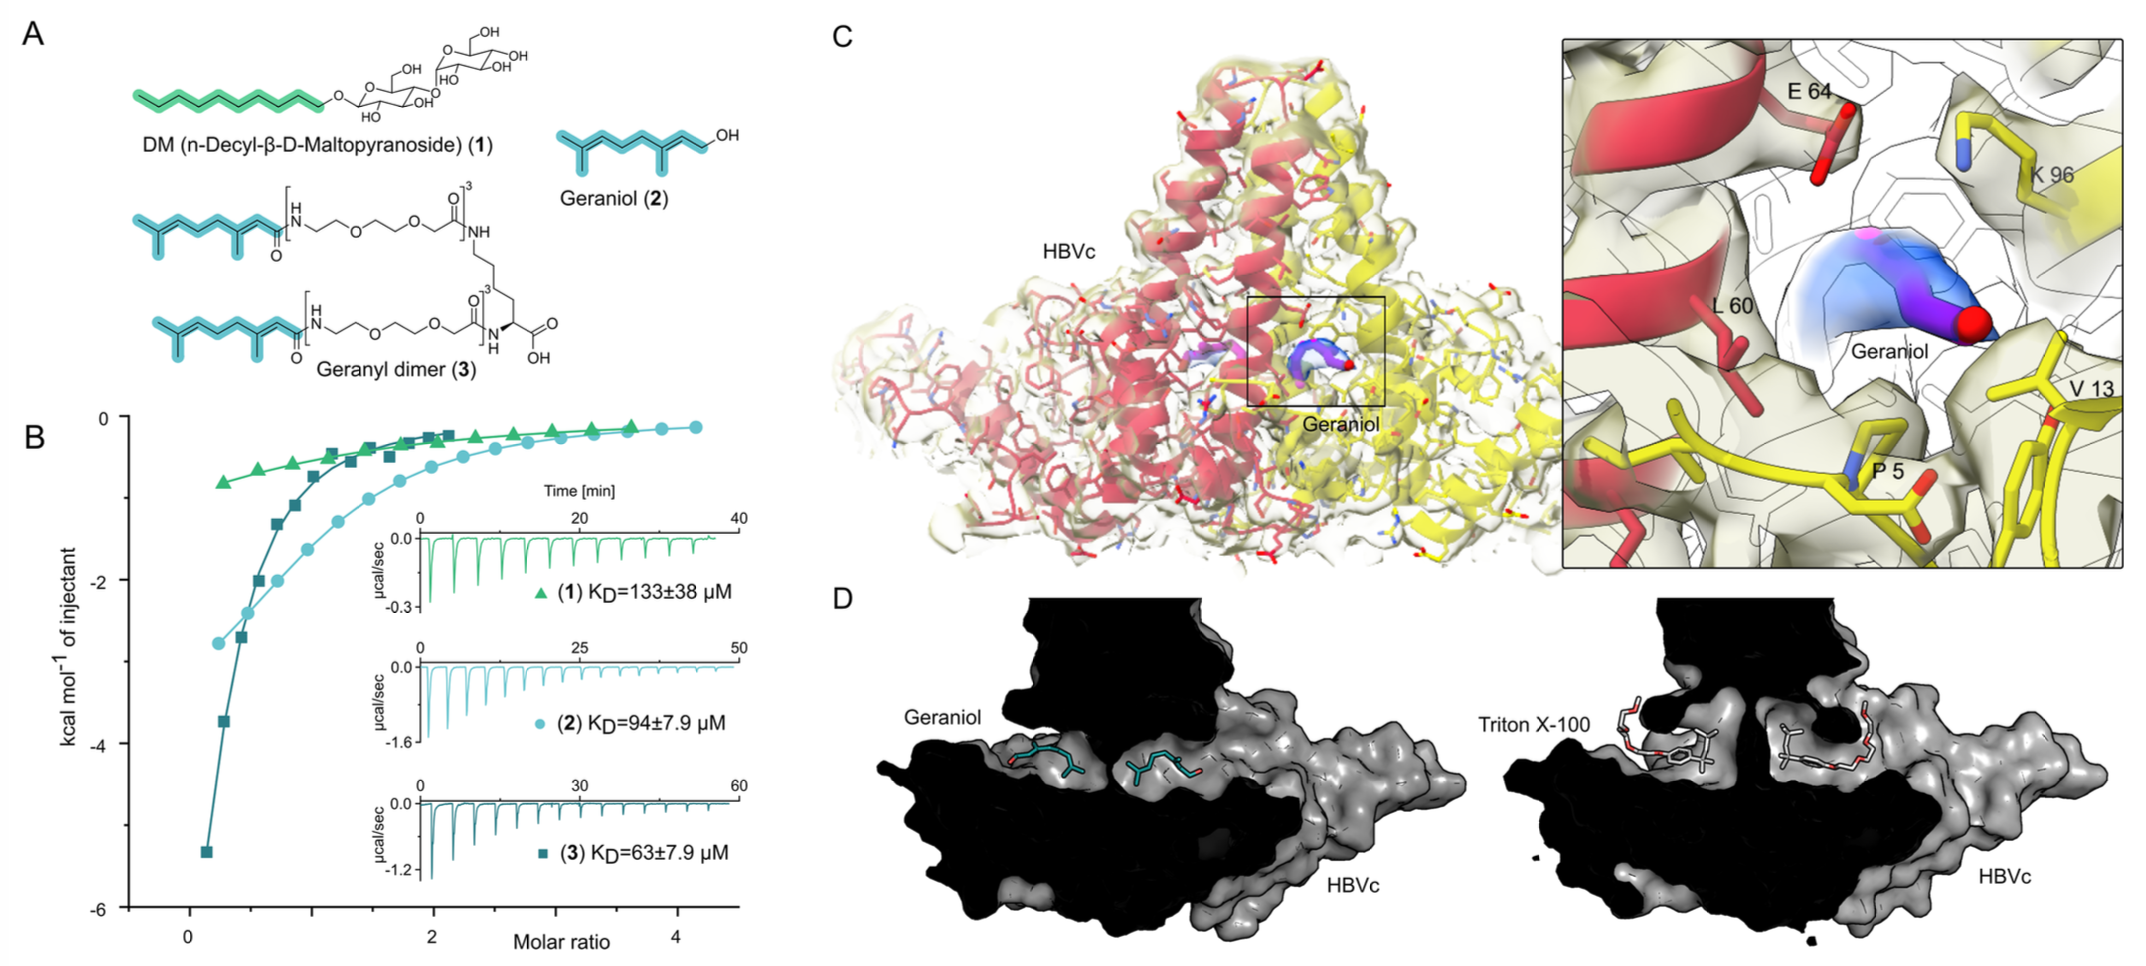
\includegraphics[width=0.82\textwidth]{figures/introduction/khayenko2024_geraniol_hbc_pocket.png}
  \caption{香叶醇（geraniol）结合HBc中心疏水口袋及其与TX100结合位点的比较。结构和热力学数据支持geraniol可与HBc核心蛋白直接相互作用，并结合在可容纳疏水分子的特定口袋中。图片截取自Khayenko等的研究\cite{khayenko2024induction}。}
  \label{fig:khayenko2024-geraniol-pocket}
\end{figure}

在上述已发表口袋结合研究的基础上，本实验室尚未发表的pull-down实验进一步检测了TX100和geraniol是否会影响preS 87--114与HBV core的体外结合。在Strep-tag pull-down实验中，研究者先将HBV core与TX100或geraniol预孵育，再加入带Strep标签的三聚化preS 87--114构建体；结果显示，在preS和输入core信号仍可检测的条件下，小分子处理组pull-down中的anti-core信号明显降低。这一结果支持TX100和geraniol在该体外体系中能够削弱preS 87--114对core的结合。由于该部分数据仍处于投稿阶段，本文仅将其作为本实验室未发表的初步机制性证据进行谨慎表述，不将其列入参考文献。

\begin{figure}[htbp]
  \centering
  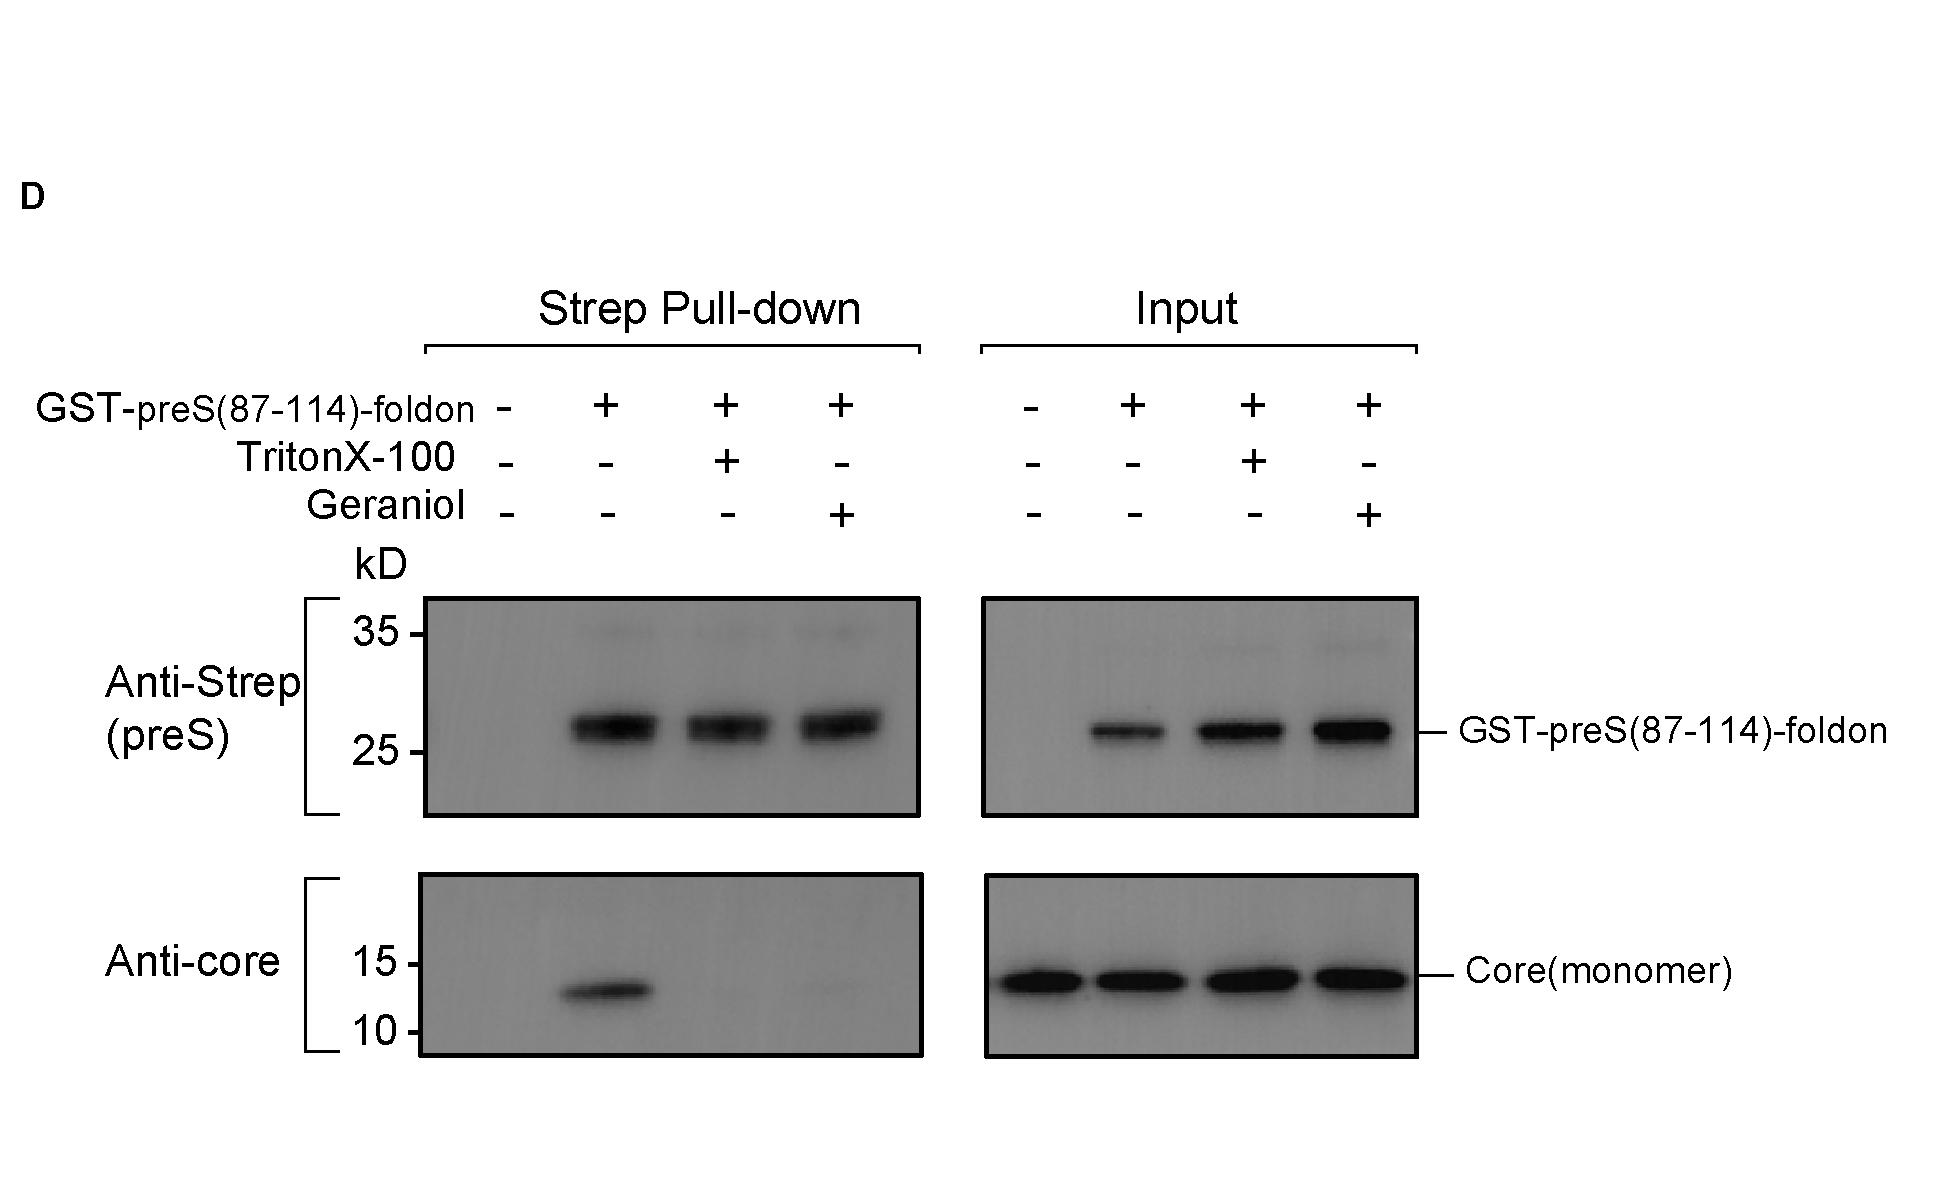
\includegraphics[width=0.68\textwidth]{figures/introduction/lab_unpublished_fig4d_pulldown_small_molecules.png}
  \caption{TX100和geraniol抑制preS 87--114--HBc体外结合的pull-down证据。Strep-tag pull-down显示，核心蛋白经TX100或geraniol预孵育后，随preS 87--114被拉下的anti-core信号降低，而输入样品中的核心蛋白和preS信号仍可检测。该图来自本实验室尚未发表的投稿中研究，因此不列入参考文献。}
  \label{fig:lab-unpublished-small-molecule-pulldown}
\end{figure}

这些发现使HBc--preS界面从单纯的病毒形态发生机制问题进一步转化为潜在药物靶点问题：若小分子能够稳定占据或调控该口袋，就可能阻断包膜化所需的关键识别步骤，从而减少感染性病毒颗粒形成。

从药物开发角度看，当前核心蛋白相关策略主要集中于衣壳组装调节剂（capsid assembly modulators, CAMs）。CAMs通过结合HBc二聚体界面附近的口袋影响核心蛋白装配、核衣壳稳定性或pgRNA封装，从而抑制病毒复制\cite{taverniti2022capsid,luo2021core}。然而，HBc不仅是衣壳组装单元，也是成熟核衣壳被包膜选择性识别的表面平台。与直接扰动衣壳组装不同，靶向HBc--preS界面有望选择性干预病毒生命周期后期的包膜化步骤，为核心蛋白靶向药物提供另一种机制类型。

既往小分子筛选研究已经证明，阻断核心蛋白与表面蛋白之间的相互作用具有可行性。Asif-Ullah等通过ELISA检测HBc与preS结合并筛选化合物，发现部分小分子能够抑制该相互作用，并降低细胞中HBV颗粒释放水平\cite{asifullah2006compounds}。虽然这些早期化合物距离临床药物仍有较大距离，但它们从概念上证明了核衣壳--包膜蛋白界面具有可干预性。TX100和geraniol的HBc口袋结合研究则进一步提示，后续药物设计可以围绕HBc表面可成药口袋、竞争机制和体外互作验证进行理性优化。

从生物安全和实验可控性角度看，利用非感染性重组蛋白、合成片段或报告系统研究HBc--preS结合，是解析该界面和评估候选抑制物的合适路径。此类体系不涉及感染性病毒扩增或病毒传播能力增强，而是将问题聚焦于纯化组分之间的物理相互作用及其抑制规律。对于毕业论文研究而言，建立稳健的体外定量平台，比较preS 87--114相关构建体和小分子竞争效应，既能够服务于基础机制研究，也能够为后续更严格的药物筛选和细胞水平验证提供前期依据。

\section{本研究的目的与意义}

综上所述，HBc--preS相互作用是HBV感染性颗粒形成中的关键步骤，也是连接结构生物学机制研究与新型抗病毒药物开发的重要界面。已有遗传学、生化和细胞实验表明preS区域参与核衣壳包膜化；Bruss的功能定位研究进一步支持preS 87--114是与core发生关键相互作用的区域\cite{bruss1997short}。同时，TX100和geraniol等小分子能够结合HBc特定疏水口袋，为探索小分子干预HBc--preS相互作用提供了依据。该方向仍需要更多定量实验支持，特别是在不同preS构建体和不同小分子浓度条件下，对HBc--preS结合强弱进行系统比较。

本研究旨在建立并应用基于NanoBiT的HBc--preS体外定量检测平台，在安全、可控的非感染性重组蛋白体系中验证HBV核衣壳与HBsAg preS区域的相互作用。研究重点包括：比较野生型与突变preS片段的HBc结合能力；评估Triton X-100、geraniol等小分子对HBc--preS相互作用的抑制效果；并结合已发表口袋结合研究和本研究体外实验结果解释小分子竞争所反映的界面机制。通过这些工作，可以进一步验证preS 87--114与HBc相互作用在HBV包膜化中的功能意义，为靶向核衣壳--包膜蛋白相互作用的新型抗病毒策略提供实验依据。

\chapter{实验基础与研究方法}

\section{实验体系设计与技术路线}

本研究建立HBV核心蛋白（HBc）与HBsAg preS区域相互作用的体外检测体系，并将其用于preS突变体和候选小分子的比较。为保证实验过程安全可控，本文所有实验均使用非感染性重组蛋白、人工构建的融合蛋白和体外发光检测体系，不涉及感染性HBV颗粒扩增、病毒传播能力增强或细胞感染模型。实验对象限定为HBc与preS片段之间的物理相互作用，而不是完整病毒复制过程。

既往遗传学和结构研究将preS 87--114片段指向L-HBsAg介导病毒颗粒形成的短线性功能区附近，该片段可能参与preS对HBV核衣壳的识别。本研究先尝试ELISA检测，比较不同固定化方式对HBc--preS互作读数的影响；随后使用NanoBiT发光互补体系，在溶液状态下检测HBVCp182与preS 87--114片段之间的空间接近。经过蛋白纯化、构建体设计、对照设置和检测条件调整后，后续小分子抑制和preS突变体比较主要采用NanoBiT方法。

实验路线从蛋白制备开始。本文表达并纯化HBVCp149、StrepXT、抗HBc抗体以及HBVCp182-SmBiT、LgBiT-preS等融合蛋白，再依次比较HBc直接包被、StrepXT捕获preS和抗HBc Fab捕获HBc三种ELISA模式。NanoBiT部分则比较含foldon三聚化结构域、不含foldon三聚化结构域以及去除GST标签后的构建体条件。最后，利用优化后的体系检测Triton X-100、香叶醇等小分子以及preS R102A、H105A、W111A突变体对HBc--preS结合的影响。

\section{重组蛋白表达、纯化与质量分析}

\subsection{HBVCp149的表达与纯化}

HBVCp149用于ELISA中的核心蛋白包被或捕获实验。将HBV核心蛋白表达质粒转化至\textit{E. coli} NiCo21(DE3)感受态细胞，在含相应抗生素的LB培养基中培养。当菌液OD$_{600}$达到0.6--0.8时，加入200 \textmu M IPTG诱导表达，并在37 ℃继续培养4 h。收集菌体后用TBS洗涤，并以含PMSF、溶菌酶、核酸酶和MgCl$_2$的裂解缓冲液重悬。样品经反复冻融裂解后离心去除不溶物。

澄清上清首先进行硫酸铵分级沉淀。通过加入3.5 M硫酸铵溶液，将体系硫酸铵浓度调至15\%，去除部分杂质；随后继续提高至45\%，沉淀HBV核心蛋白颗粒。沉淀用20 mM Tris（pH 8.0）重悬后，经Q HP阴离子交换柱进一步纯化。层析使用ÄKTA系统，以低盐缓冲液上样，并用含1 M NaCl的Q-B缓冲液进行线性梯度洗脱。收集含HBVCp149的组分，用SDS-PAGE评估纯度后合并，用于后续ELISA实验。

\subsection{StrepXT的表达、复性与功能评估}

StrepXT用于定向捕获带Strep标签的preS蛋白。将StrepXT表达质粒转化至\textit{E. coli} NiCo21-pLysS细胞，在含卡那霉素和氯霉素的LB培养基中培养。当OD$_{600}$达到0.6--0.8时，加入1 mM IPTG诱导，并在37 ℃培养4 h。收集菌体后用含EDTA的TBS洗涤并冻存。

纯化时将菌体沉淀在含EDTA和Triton X-100的Tris缓冲液中重悬，经冻融、核酸酶处理和超声破碎后离心。StrepXT主要以包涵体形式存在，因此对沉淀进行洗涤后，用6 M盐酸胍在酸性条件下溶解，并通过透析逐步复性。复性后的样品经离心和过滤后上样至Q柱，以NaCl梯度洗脱。含目标条带的组分经SDS-PAGE确认后用于后续实验。为确认StrepXT复性后仍具备功能，进一步测定其Strep标签结合能力，并据此确定其可用于preS捕获ELISA。

\subsection{抗HBc IgG的转染与纯化}

为改善ELISA中核心蛋白检测或捕获步骤，本研究使用抗HBc抗体材料。抗HBc IgG通过重链和轻链质粒共转染OPM细胞获得。转染后12--24 h加入丁酸钠促进表达，并继续培养约5 d。收集细胞培养上清后，加入咪唑、Tris和NaCl调节缓冲条件，并使用Ni-NTA树脂进行纯化。样品经上样、流穿回收、低浓度咪唑洗涤和高浓度咪唑洗脱后，收集洗脱组分。纯化产物通过还原和非还原SDS-PAGE分析，以判断重链、轻链和完整IgG条带是否符合预期。合并的IgG洗脱组分经浓缩和换液后用于ELISA检测。

\subsection{HBVCp182-SmBiT融合蛋白的表达与纯化}

核心蛋白侧构建体记为HBVCp182-\allowbreak{}SmBiT。将编码该融合蛋白的质粒转化至\textit{E. coli} NiCo21细胞，在含氨苄青霉素的LB培养基中培养。当OD$_{600}$达到0.6--0.8时，用200 \textmu M IPTG诱导表达，37 ℃培养4 h。收集菌体后用TBS洗涤，并可经液氮速冻后保存于-80 ℃。

初始纯化采用冻融裂解、硫酸铵分级沉淀和Q HP阴离子交换层析。菌体沉淀用含PMSF、溶菌酶、核酸酶和MgCl$_2$的TBS裂解缓冲液重悬，经冻融裂解后离心。上清经硫酸铵沉淀富集目标蛋白，沉淀用20 mM Tris（pH 8.0）重悬，并稀释降低电导后上样至Q HP阴离子交换柱，以盐梯度洗脱。纯化后的组分通过SDS-PAGE和anti-HBcAg蛋白质印迹（Western blot）检测确认目标条带，并通过NanoBiT活性比较筛选可用于后续实验的合并组分。

\subsection{LgBiT-preS融合蛋白、阴性对照和阳性对照的制备}

NanoBiT实验还需要三类配套蛋白：含preS 87--114片段的LgBiT融合蛋白，不含preS的LgBiT阴性对照，以及用于验证互补体系的GST-SmBiT阳性对照相关蛋白。早期实验采用GST-LgBiT-preS 87--114-foldon-strep-His和对应的GST-LgBiT-foldon-strep-His阴性对照，利用foldon三聚化结构域提高preS片段的多价呈递。由于foldon三聚化和GST二聚化都可能改变表观结合强度，后续又制备了不含foldon三聚化结构域的GST-LgBiT-preS 87--114-His和GST-LgBiT-His。

三种GST标记融合蛋白均在\textit{E. coli} NiCo21中表达。菌液OD$_{600}$达到0.6--0.8后加入200 \textmu M IPTG，在16 ℃诱导12 h。收集菌体后以含Tris、NaCl、PMSF、核酸酶和MgCl$_2$的裂解缓冲液重悬，并在冰浴中超声破碎。离心澄清后，上清上样至GST亲和柱。柱子经高盐缓冲液和TBS洗涤后，用含还原型谷胱甘肽的洗脱缓冲液洗脱目标蛋白。

对于GST-LgBiT-preS 87--114-His和GST-LgBiT-His回收效率较低的情况，改进纯化方法，依次通过Ni亲和柱和Q HP阴离子交换柱得到纯化蛋白，以获得足量实验组和阴性对照蛋白。

部分GST-LgBiT融合蛋白用PPase去除GST标签，以减少GST二聚化对NanoBiT读数的干扰。酶切前后通过SDS-PAGE比较迁移率，并依据GST、LgBiT-preS和LgBiT条带判断酶切是否充分。去除GST标签后的蛋白用于比较野生型preS与突变体的HBc结合能力。

\section{ELISA检测体系}

\subsection{ELISA检测原理与类型}

酶联免疫吸附实验（enzyme-linked immunosorbent assay, ELISA）属于固相免疫检测方法，核心是抗原--抗体识别和酶催化信号放大。常规ELISA先把抗原或抗体固定在聚苯乙烯等载体表面，再通过封闭步骤减少非特异性吸附。随后依次加入待测样品、识别抗体和酶标试剂，洗去未结合组分后，由辣根过氧化物酶或碱性磷酸酶等酶标分子催化底物显色或发光。读数强弱可反映待测抗原或抗体的相对含量\cite{aydin2015short,ahirwar2022unveiling}。ELISA常用于蛋白、抗原、抗体和其他生物标志物检测\cite{ahirwar2022unveiling}。

按抗原、抗体和酶标试剂的组合方式，ELISA可分为直接、间接、夹心和竞争四类（图\ref{fig:elisa-types}）。直接ELISA把抗原固定在板面，用酶标一抗读取信号，流程短，但放大能力有限。间接ELISA同样先固定抗原，再用未标记一抗识别目标，最后加入酶标二抗，因此信号放大更明显，试剂搭配也更灵活。夹心ELISA先由捕获抗体固定待测抗原，再用识别另一表位的检测抗体和酶标二抗产生信号，适用于对特异性和灵敏度要求较高的检测。竞争ELISA利用样品中的待测物与酶标竞争物争夺有限结合位点，读数通常与待测物浓度呈反向关系，常用于小分子、单表位抗原或难以被两种抗体同时识别的目标\cite{aydin2015short,ahirwar2022unveiling}。

\begin{figure}[htbp]
  \centering
  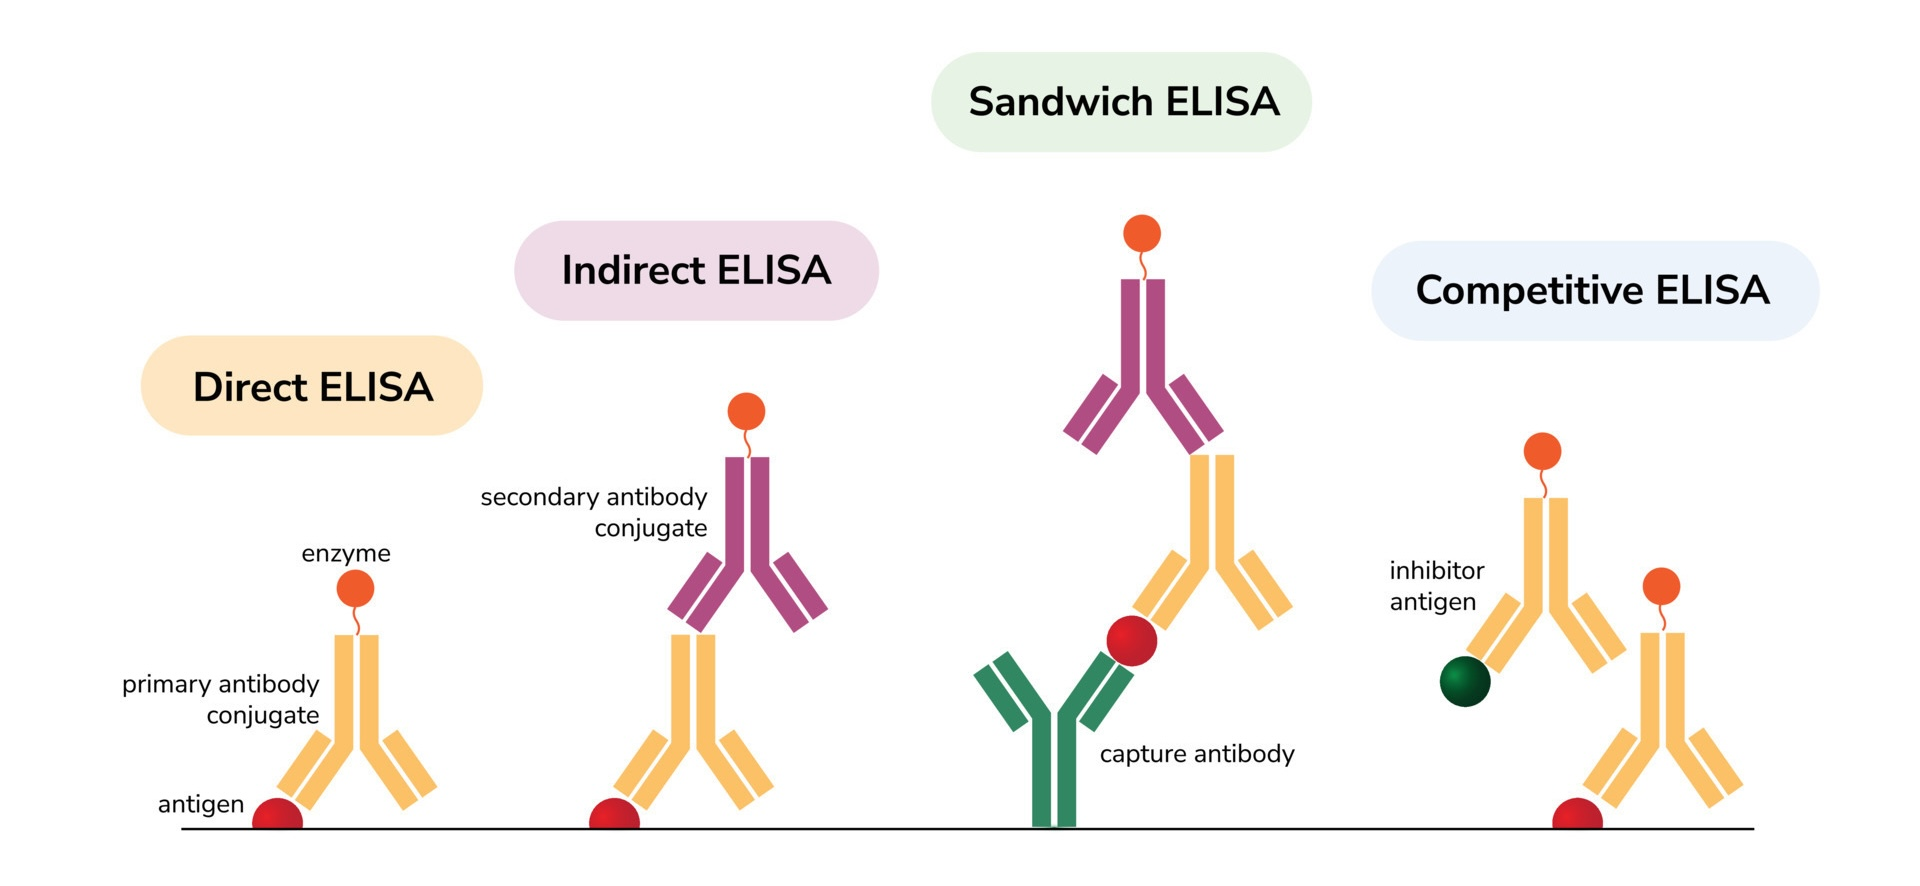
\includegraphics[width=0.95\textwidth]{figures/methods/elisa_types.jpg}
  \caption{四种ELISA类型示意。直接、间接、夹心和竞争ELISA在抗原固定、抗体识别和酶标读出方式上不同，均把抗原--抗体结合转换为酶促信号。图片来源vecteezy。}
  \label{fig:elisa-types}
\end{figure}

\subsection{HBc直接包被ELISA}

HBc直接包被ELISA用于观察preS能否与固定化HBc结合。实验中先将HBVCp149直接吸附到酶标板，封闭后加入带标签的preS蛋白，再用抗标签抗体和显色体系读取板上preS信号。

先对HBVCp149包被浓度进行滴定，并用Langmuir单点吸附模型拟合总信号和特异信号，据此选择后续实验的工作包被浓度。随后在固定HBVCp149的条件下滴定preS，同时设置无HBc包被对照，用来区分HBc依赖性信号和preS或抗体带来的非特异吸附背景。

\subsection{StrepXT捕获preS ELISA}

StrepXT捕获preS ELISA用于调整preS在固相表面的取向。实验时先用StrepXT包被酶标板，封闭后加入带Strep标签的preS蛋白，使preS通过标签被定向捕获；随后加入HBVCp149，并利用抗HBc抗体读取与preS结合的核心蛋白信号。

实验流程先优化StrepXT包被和preS捕获条件，再对preS进行浓度滴定，并用Langmuir模型拟合捕获曲线。根据preS捕获饱和趋势确定工作浓度后，继续滴定HBVCp149，比较实验组与无preS对照组的信号差异。为提高核心蛋白检测灵敏度，后续实验以纯化得到的抗HBc IgG D4替代初始检测抗体。

\subsection{抗HBc Fab捕获HBc ELISA}

抗HBc Fab捕获HBc ELISA用于改善HBc固定化方式。实验中先将抗HBc Fab包被于酶标板，再加入HBVCp149，使核心颗粒由抗体捕获；随后加入preS蛋白，并通过抗GST抗体检测preS信号。该构型避免HBc直接吸附到塑料表面，理论上更有利于保留核心颗粒构象。

实验中先滴定HBVCp149以确定Fab捕获效率和合适核心蛋白浓度，再在固定HBc条件下滴定preS，并设置无HBc和仅HRP对照等对照以评估背景来源。

\begin{figure}[htbp]
  \centering
  \begin{minipage}{0.42\textwidth}
    \centering
    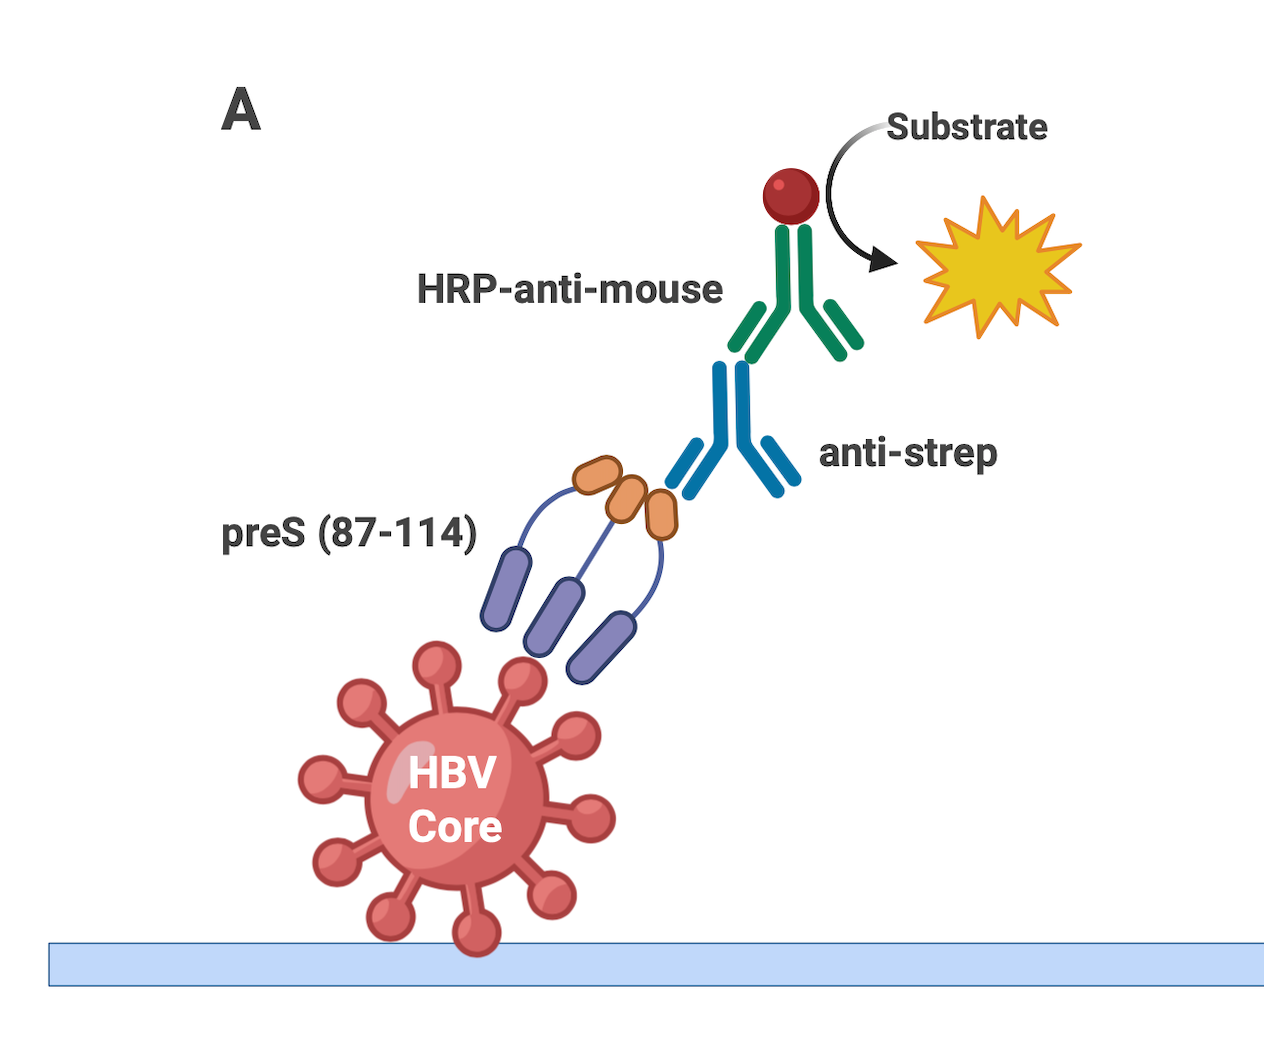
\includegraphics[width=\textwidth]{figures/methods/elisa_a.png}
  \end{minipage}
  \hspace{0.07\textwidth}
  \begin{minipage}{0.42\textwidth}
    \centering
    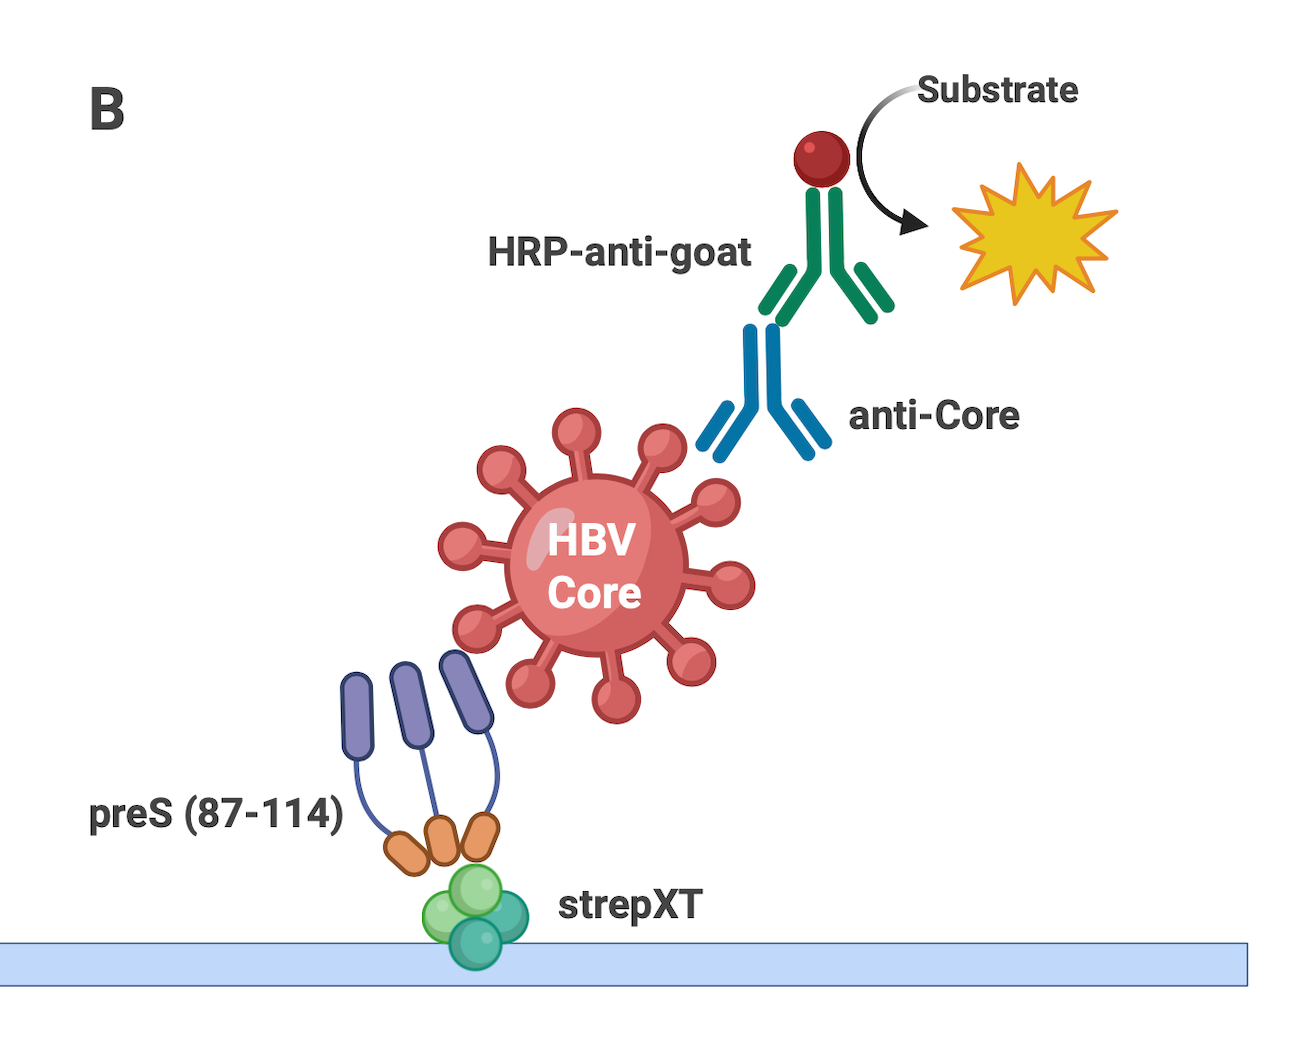
\includegraphics[width=\textwidth]{figures/methods/elisa_b.png}
  \end{minipage}
  \par\medskip
  \begin{minipage}{0.46\textwidth}
    \centering
    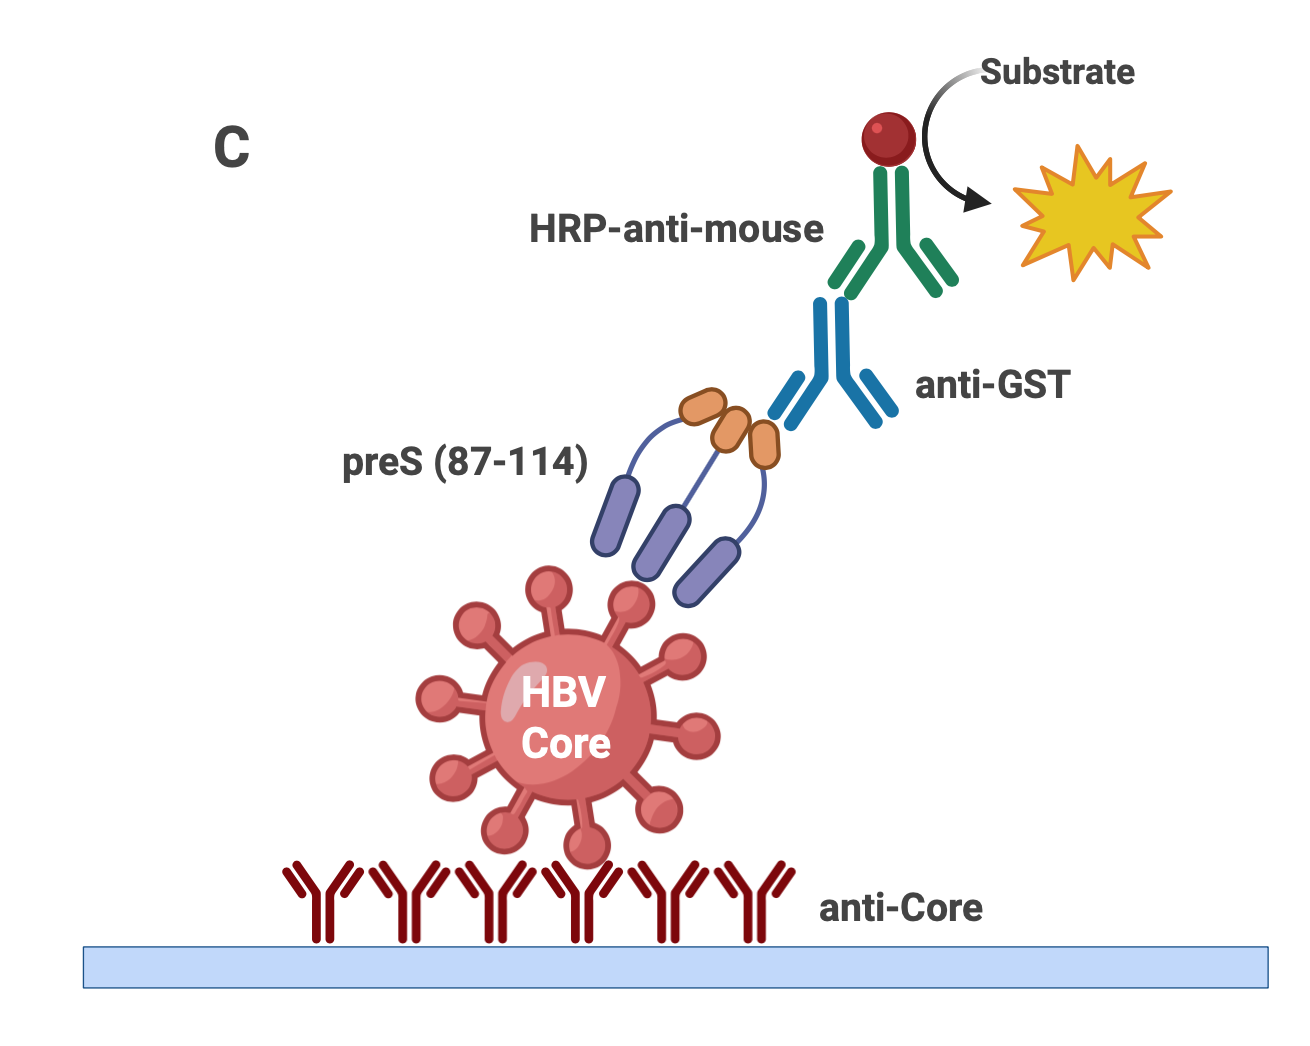
\includegraphics[width=\textwidth]{figures/methods/elisa_c.png}
  \end{minipage}
  \hspace{0.04\textwidth}
  \begin{minipage}{0.42\textwidth}
    \centering
    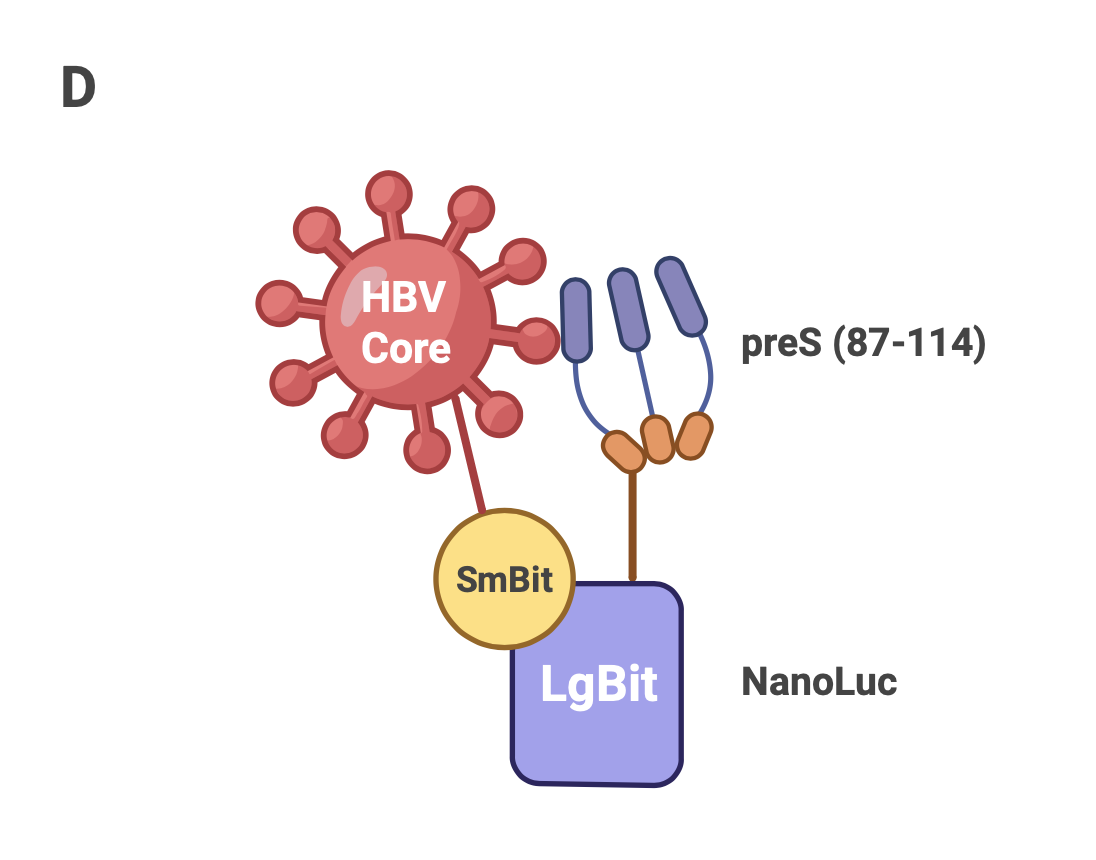
\includegraphics[width=\textwidth]{figures/methods/nanobit.png}
  \end{minipage}
  \caption{HBc--preS相互作用检测模式。A，HBc直接包被ELISA：HBVCp149固定于酶标板，再加入preS 87--114融合蛋白，并通过抗标签抗体及HRP显色体系检测preS信号。B，StrepXT捕获preS ELISA：StrepXT固定在板面后捕获带Strep标签的preS 87--114融合蛋白，再加入HBVCp149，并通过抗HBc抗体及HRP显色体系检测核心蛋白信号。C，抗HBc Fab捕获HBc ELISA：抗HBc Fab固定于酶标板并捕获HBVCp149，再加入preS 87--114融合蛋白，并通过抗GST抗体及HRP显色体系检测preS信号。D，NanoBiT发光互补检测：SmBiT位于HBVCp182侧，LgBiT位于preS 87--114侧；二者接近时恢复NanoLuc活性，加入底物后产生发光信号。}
  \label{fig:method-assay-formats}
\end{figure}

\section{NanoBiT发光互补检测}

\subsection{NanoBiT技术原理}

NanoBiT是一种基于NanoLuc荧光素酶拆分互补的蛋白相互作用检测技术。NanoLuc是一种小分子、单体化且发光强度较高的工程化荧光素酶，可催化furimazine氧化生成furimamide、二氧化碳和光信号。Dixon等利用NanoLuc体积小和发光强的特点，将其工程化拆分为两个互补片段：较大的LgBiT片段约18 kDa，较小的SmBiT片段为11个氨基酸、约1.3 kDa\cite{dixon2016nanoluc}。LgBiT与SmBiT单独存在时自发亲和力较弱；当二者分别融合到两个待测蛋白上，并因目标蛋白相互作用而靠近时，LgBiT和SmBiT可发生结构互补，重新形成具有催化活性的NanoLuc复合物，加入底物后产生发光信号。

\begin{figure}[htbp]
  \centering
  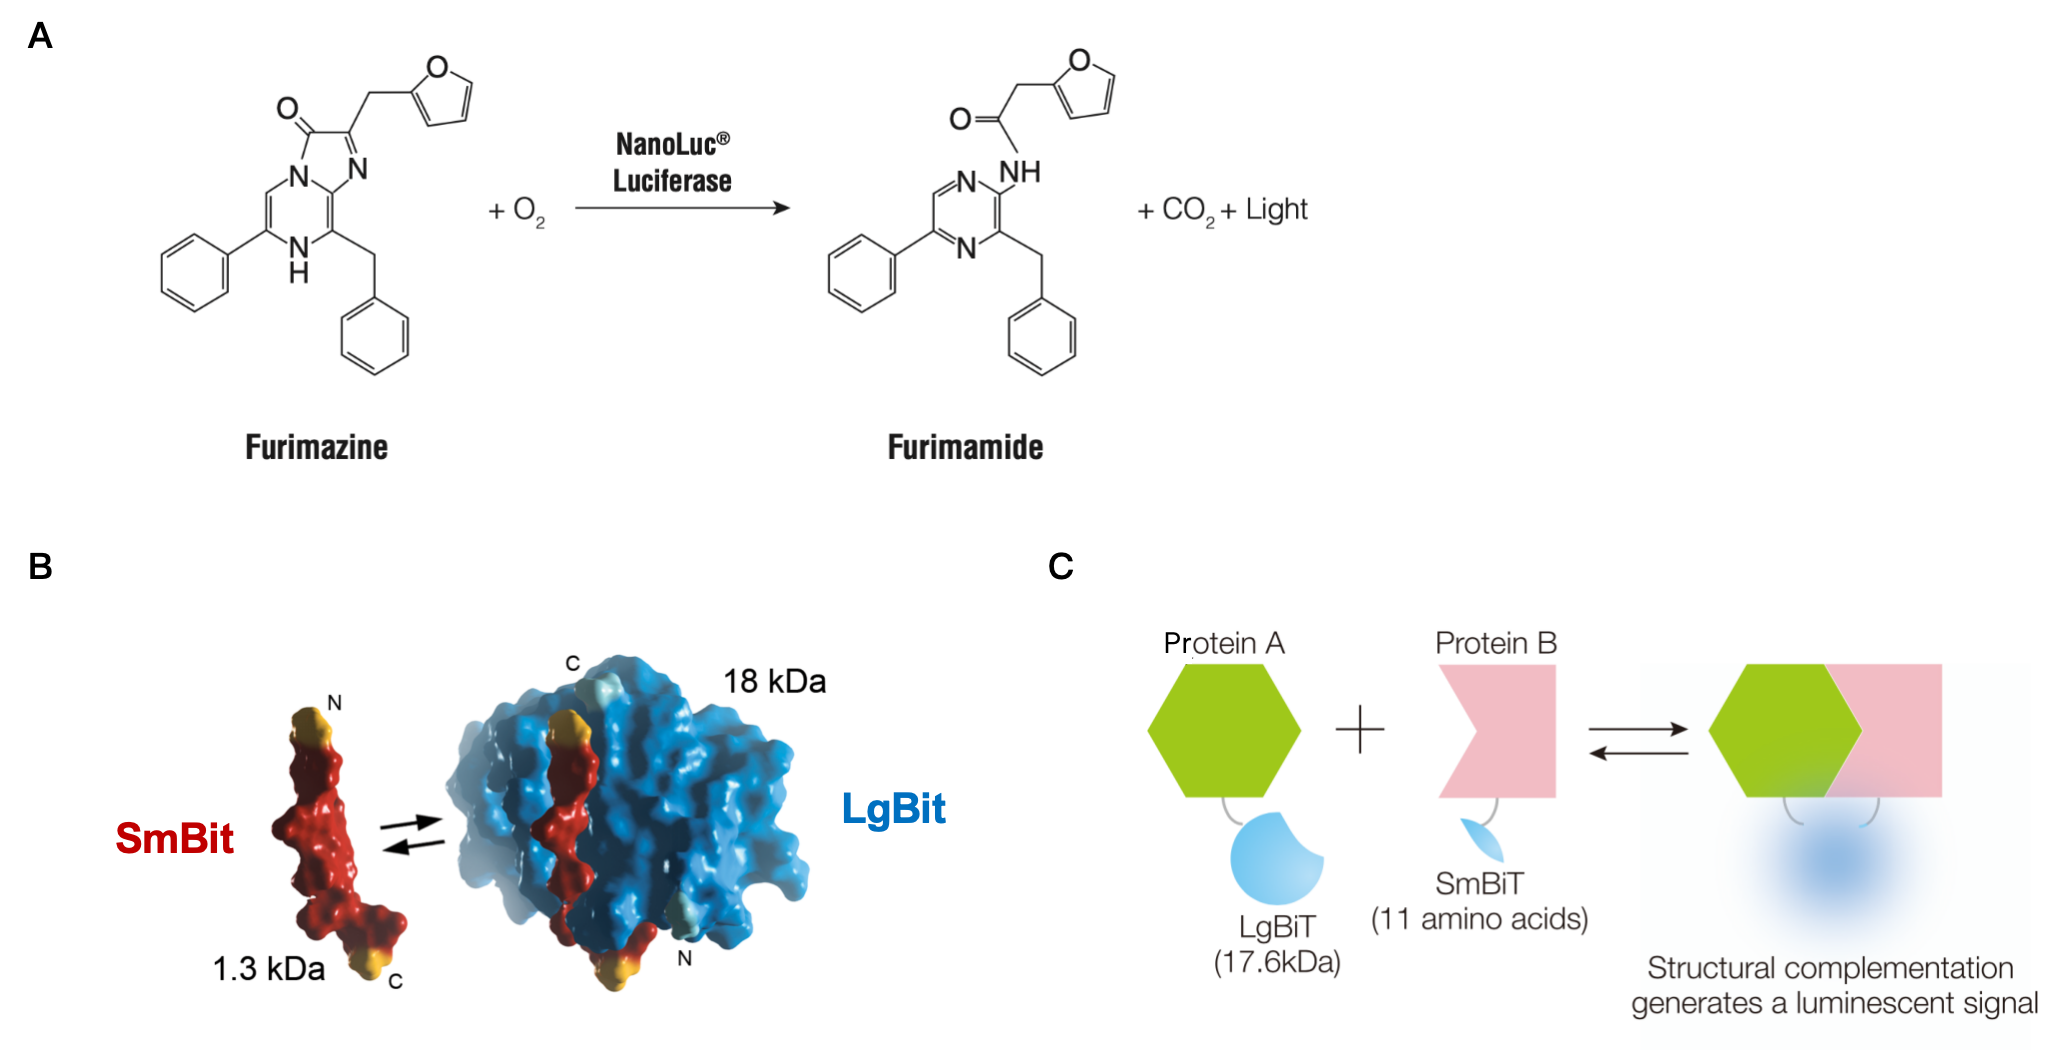
\includegraphics[width=0.75\textwidth]{figures/introduction/nanobit_principle.png}
  \caption{NanoLuc与NanoBiT蛋白互补技术原理。A，NanoLuc催化furimazine氧化并产生发光信号。B，NanoBiT由SmBiT和LgBiT组成，二者互补后恢复NanoLuc活性。C，SmBiT和LgBiT分别融合到两个待测蛋白上时，目标蛋白靠近可带来发光信号。\cite{dixon2016nanoluc}。}
  \label{fig:nanobit-principle}
\end{figure}

与传统亲和沉淀、免疫共沉淀或ELISA相比，NanoBiT读数来自两个融合蛋白在溶液或细胞环境中的空间接近，不必把相互作用完全限制在固相表面。检测过程中也不需要多轮洗涤，因此更接近溶液状态，适合观察HBc--preS这类较弱、可逆且可能受固定化影响的相互作用。Dixon等测得NanoBiT片段自身的本征亲和力约为190 \textmu M，互补过程具有可逆性；这一设计可降低报告片段自身结合对待测蛋白相互作用的驱动作用\cite{dixon2016nanoluc}。NanoLuc体系发光强、背景低、线性范围宽，便于在多孔板中做定量检测和候选调节因子筛选。

\subsection{NanoBiT构建体设计}

构建体设计时，较大的LgBiT不放在HBc侧，以免干扰HBc组装。本研究把较小的SmBiT融合至HBVCp182，把LgBiT接到preS 87--114片段一侧。实验组为HBVCp182-SmBiT与LgBiT-preS 87--114组合；阴性对照为HBVCp182-SmBiT与不含preS的LgBiT融合蛋白组合；阳性对照利用GST标签二聚化特性，将GST-SmBiT与GST-LgBiT相关蛋白组合，用来确认NanoBiT报告系统的检测上限。需要说明的是，NanoBiT信号本质上反映融合蛋白之间的近距离互补，因此仍需结合阴性对照、标签方向、蛋白质量控制以及小分子对发光体系本身影响的排查，再谨慎解释HBc--preS相互作用或其抑制效应。

\subsection{NanoBiT发光检测流程}

NanoBiT检测在白色384孔板中进行。实验前将LgBiT融合蛋白和SmBiT融合蛋白分别用TBS稀释为合适浓度。常规反应中，将10 \textmu L LgBiT融合蛋白与10 \textmu L SmBiT融合蛋白混合，使总体积为20 \textmu L。混合后短暂离心，并在室温孵育约10 min。随后加入20 \textmu L新鲜配制的Nano-Glo底物工作液，底物与缓冲液按1:50配制。加样后振荡约10 s，在室温孵育3--5 min，并使用酶标仪读取发光信号，积分时间设为1000 ms。

初始NanoBiT实验中，LgBiT与SmBiT蛋白按1:1浓度比例混合，以判断实验组、阴性对照和阳性对照之间是否存在可分辨信号。优化实验中固定HBVCp182-SmBiT的终浓度，并滴定LgBiT-preS或LgBiT阴性对照蛋白。

\section{小分子抑制、突变体比较与数据分析}

\subsection{小分子抑制实验}

小分子抑制实验用于评估候选分子是否改变HBc--preS相关NanoBiT信号。本文检测Triton X-100（TX100）、NP-40和香叶醇。在含foldon三聚化结构域的体系中，根据NanoBiT滴定结果选择40 nM GST-LgBiT-preS 87--114-foldon-strep-His作为初筛工作浓度，并使用相同浓度的GST-LgBiT-foldon-strep-His作为阴性对照。初筛时，将小分子按浓度梯度加入NanoBiT反应体系后读取发光信号。由于直接加药条件下抑制趋势不够稳定，后续改为先将小分子与HBVCp182-SmBiT预孵育约2 h，再加入LgBiT-preS或LgBiT阴性对照检测，并适当提高小分子浓度范围。分析这些结果时，同时考虑溶剂背景、高浓度去垢剂对蛋白稳定性、NanoBiT片段互补、底物发光反应和体系浊度的影响。

为降低foldon三聚化结构域带来的多价效应，后续构建并制备不含该结构域的GST-LgBiT-preS 87--114-His和GST-LgBiT-His。该体系主要用于观察去除foldon三聚化结构域后NanoBiT信号窗口如何变化，并作为preS突变体比较的基础；本文的小分子表观抑制结果仍主要基于含foldon三聚化结构域的构建体解释。实验中同步检测实验组和阴性对照组，分析时扣除或比较阴性对照背景，以判断小分子对HBc--preS相关信号的影响。

\subsection{preS突变体结合能力比较}

为检验结构模型中关键残基对HBc结合的贡献，本研究比较野生型（wild-type）preS 87--114及R102A、H105A和W111A突变体的NanoBiT信号。由于foldon三聚化结构域和GST标签可能带来多价结合或非目标性二聚化，突变体比较优先使用去除foldon三聚化结构域后的LgBiT-preS蛋白。实验中固定HBVCp182-SmBiT，滴定不同LgBiT-preS突变体蛋白，并设置LgBiT阴性对照。通过比较同一浓度范围内的发光信号强度和相对趋势，评估各残基对HBc--preS相互作用的影响。

\subsection{数据处理与评价指标}

ELISA和NanoBiT实验均设置实验组、阴性对照和必要的背景对照。对于浓度滴定实验，首先计算各条件下重复孔的平均值和标准差；除特别说明外，图中误差线表示同一实验内重复孔的标准差。随后根据实验设计扣除无核心蛋白、无preS或不含preS的LgBiT阴性对照背景，得到特异性信号。对呈饱和趋势的结合曲线，可采用Langmuir单点结合模型进行拟合，以描述信号随蛋白浓度增加逐渐接近平台的趋势。由于NanoBiT读数同时受到融合蛋白空间接近、片段互补效率和标签多聚化状态影响，拟合参数仅作为当前检测构型下的表观参数，不直接等同于热力学解离常数。

检测体系的统计学窗口使用Z-factor评价。Z-factor同时考虑实验组与阴性对照之间的均值差异和组内波动，可反映检测体系是否具备稳定筛选能力，其计算公式如下\cite{zhang1999simple}：
\begin{equation}
  Z = 1 - \frac{3\left(\sigma_{\mathrm{exp}}+\sigma_{\mathrm{neg}}\right)}
  {\left|\mu_{\mathrm{exp}}-\mu_{\mathrm{neg}}\right|}.
  \label{eq:z-factor}
\end{equation}
其中，$\mu_{\mathrm{exp}}$和$\sigma_{\mathrm{exp}}$分别表示实验组信号的平均值和标准差，$\mu_{\mathrm{neg}}$和$\sigma_{\mathrm{neg}}$分别表示阴性对照信号的平均值和标准差。通常Z-factor大于0.5说明检测窗口较好，可用于较稳健的定量比较；0--0.5提示体系处于边界状态；小于0则说明实验组和对照组分离不足或波动过大。Z-factor反映筛选窗口质量，不能单独证明分子机制。小分子抑制实验中，若高浓度小分子同时改变阴性对照信号、阳性互补信号或底物背景，则不直接计算IC$_{50}$，仅进行趋势性分析，并把背景变化列为后续优化内容。

\chapter{实验结果与分析}

\section{ELISA检测体系的建立与评价}

\subsection{ELISA检测体系的设计思路}

本研究的核心目标是建立能够定量反映HBV核心蛋白（HBc）与HBsAg preS区域相互作用的体外检测体系，并为后续比较preS突变体及小分子抑制剂的影响奠定基础。根据前期结构研究，preS 87--114片段是与HBV核衣壳结合的关键区域。因此，本研究首先围绕HBc与preS片段的互作检测进行了方法学探索。

考虑到HBc--preS相互作用可能较弱，且容易受到固定化方式、蛋白取向和洗涤步骤影响，本研究前期比较了多种ELISA模式。三类ELISA体系分别从不同角度优化互作检测：其一，直接包被HBc颗粒，再检测结合到HBc上的preS；其二，通过StrepXT定向捕获带Strep标签的preS，再加入HBc并检测结合的核心蛋白；其三，通过抗HBc Fab捕获HBc颗粒，再检测preS结合。通过比较这些模式的信号窗口、背景水平和重复性，可以判断传统固相ELISA是否适合作为后续突变体和小分子筛选平台。

\subsection{HBVCp149的表达与纯化}

为建立HBc--preS互作检测体系，首先需要获得可用于包被或捕获实验的HBV核心蛋白样品。本研究使用截短形式的HBVCp149蛋白作为实验样品。经分步盐析和Q柱阴离子层析后，HBVCp149在主要洗脱组分中呈现清晰的目标条带，说明目标蛋白得到有效富集。层析曲线中主要峰较为明显，同时伴随两个较小的肩峰，提示样品中可能存在少量不同装配状态的核心蛋白或杂质组分；但用于后续实验的合并组分在SDS-PAGE中整体较为干净，能够满足ELISA包被和定量滴定的需要。

这一结果说明，HBVCp149的表达和纯化流程可以稳定获得后续体外互作分析所需的核心蛋白材料。由于HBc的颗粒状态和表面构象对preS结合具有重要影响，后续ELISA重点比较了不同固定化方式能否在尽量保留互作界面的同时产生足够稳定的特异信号。

\begin{figure}[htbp]
  \centering
  
\includegraphics[width=1.0\textwidth]{docs/figures/result/result_01_hbvcp149.png}
  \caption{HBVCp149的表达与纯化结果。A，HBVCp149的Q HP阴离子层析柱层析曲线。B、C，不同组分的SDS-PAGE分析，目标核心蛋白在主要洗脱组分中得到富集，可用于后续ELISA检测。}
  \label{fig:hbvcp149-purification}
\end{figure}

\subsection{ELISA模式一：HBc直接包被}

在第一种ELISA模式中，HBVCp149被直接包被于酶标板表面，随后加入带标签的preS蛋白，并通过抗标签抗体检测结合到板上的preS信号。该设计的优点是检测路径较短，理论上能够直接反映preS与固定化HBc之间的结合；但其潜在问题是核心蛋白直接吸附到塑料表面后，颗粒构象或preS结合面可能受到影响，同时preS和检测抗体也可能产生非特异吸附。

首先对HBVCp149包被量进行滴定，结果显示扣除背景后的特异信号呈现可饱和趋势，且能够较好地用Langmuir单点吸附模型拟合，提示HBc直接包被在技术上具有一定可重复性。根据包被曲线，后续实验选择20 nM HBVCp149作为工作浓度。

然而，在该条件下进一步滴定preS时，实验组的特异信号仅轻微升高，整体仍接近基线；同时，在未包被HBc的对照孔中仍可保留较高的总信号。20 nM HBc组与0 nM HBc组之间分离度有限，说明该体系的读数主要受到preS或抗体在板面上的非特异吸附影响，而不是由稳定的HBc--preS特异结合主导。

\begin{figure}[htbp]
  \centering
  
\includegraphics[width=1.0\textwidth]{docs/figures/result/result_02_elisa_a.png}
  \caption{HBc直接包被的ELISA的检测结果。A、B，HBVCp149包被滴定可获得可饱和信号。C、D，在固定HBc后检测preS结合时，实验组与无HBc对照组分离有限，提示该构型受到非特异吸附背景影响。}
  \label{fig:elisa-format-a}
\end{figure}

因此，HBc直接包被ELISA虽然步骤简单，但不能提供足够清晰的HBc依赖性信号窗口。该结果提示，后续体系需要减少preS直接接触塑料表面的机会，并尽量通过定向捕获方式改善preS呈递。

\subsection{ELISA模式二：StrepXT捕获preS}

为降低preS直接吸附造成的背景，本研究进一步构建了StrepXT捕获preS的ELISA模式。在该体系中，酶标板首先包被StrepXT，随后通过Strep标签定向捕获preS，再加入HBVCp149，最后通过抗HBc抗体检测结合到preS上的核心蛋白。与直接包被HBc的体系相比，该构型的主要优势在于preS可以通过标签被定向固定，从而提高其可及性并降低随机吸附带来的背景。

首先对StrepXT进行了表达纯化和功能评估。经包涵体回收、变性复性和Q柱阴离子层析纯化后，StrepXT在洗脱组分中出现相对富集的目标条带，说明目标蛋白已从主要杂质中分离出来。进一步测定其有效结合位点，平均有效值约为0.852，提示StrepXT复性后保留了较好的Strep标签捕获能力，可用于后续preS定向固定实验。

\begin{figure}[htbp]
  \centering
  
\includegraphics[width=1.0\textwidth]{docs/figures/result/result_03_strepXT.png}
  \caption{StrepXT的表达纯化与功能评估。A，透析前各组分的SDS-PAGE分析。B，StrepXT的Q HP阴离子层析柱层析曲线。C、D，阴离子层析后各组分的SDS-PAGE分析，结果显示StrepXT在洗脱组分中得到富集；结合位点定量结果表明复性后的StrepXT具有较好的Strep标签捕获能力。}
  \label{fig:strepx-purification}
\end{figure}

在StrepXT捕获体系中，50 nM StrepXT能够较稳定地包被于板面并捕获带Strep标签的preS。preS滴定曲线呈现典型的可饱和趋势，且能够较好地用Langmuir单点吸附模型拟合，说明该体系能够有效控制preS本身的呈递过程。基于该结果，后续HBVCp149结合实验中选择100 nM preS作为工作浓度。与HBc直接包被体系相比，StrepXT捕获明显改善了preS固定化方式，说明模式一中的部分背景确实来源于preS在板面上的非特异吸附。

然而，在HBc结合实验中，核心蛋白检测信号仍然非常分散，信噪比过低，特异信号窗口几乎不可见。推测这可能是因为用于检测的抗HBc抗体的特异性过低，因此进一步制备了特异性较高的抗HBc IgG重复实验，希望可以提高信号的特异性。

\begin{figure}[htbp]
  \centering
  
\includegraphics[width=1.0\textwidth]{docs/figures/result/result_04_elisa_b_1.png}
  \caption{StrepXT捕获preS的ELISA模式的初步检测结果。A，preS捕获滴定呈现可饱和曲线，说明preS呈递得到改善。B，HBV核心蛋白结合检测的特异信号仍较弱且波动较大。}
  \label{fig:elisa-format-b-initial}
\end{figure}

SDS-PAGE结果显示，IgG D4在还原条件下具有清晰的重链和轻链条带，在非还原条件下可见完整IgG条带，说明该抗体成功表达和纯化。后续实验使用IgG D4替代原检测抗体。

\begin{figure}[htbp]
  \centering
  
\includegraphics[width=0.4\textwidth]{docs/figures/result/result_05_IgG D4.png}
  \caption{抗HBc IgG的表达与纯化结果。IgG D4在还原条件下显示重链和轻链条带，在非还原条件下显示完整IgG条带，可被用于后续HBV核心蛋白检测。}
  \label{fig:anti-core-igg}
\end{figure}

替换为抗HBc IgG D4后，100 nM preS组与0 nM preS对照组之间的分离度显著改善，尤其是在中高浓度HBVCp149条件下，实验组信号随核心蛋白浓度升高而逐渐增加，而对照组上升较慢。这表明该ELISA模式能够报告一定的preS依赖性核心蛋白结合成分。然而，该体系的动态窗口仍不稳定：绝对信号较低，低浓度点波动明显，不同浓度下计算得到的Z-factor变化较大。最佳Z-factor出现在1280 nM HBVCp149条件下，约为0.397；整体范围为-8.896至0.397，始终未达到通常认为适合稳健筛选的0.5阈值。

\begin{figure}[htb]
  \centering
  
\includegraphics[width=1.0\textwidth]{docs/figures/result/result_06_elisa_b_2.png}
  \caption{替换抗HBc IgG D4后的StrepXT捕获preS的ELISA结果。A，100nM和0nM preS包被后HBc的滴定曲线。B，HBc滴定的特异性信号。中高浓度HBVCp149条件下信噪比显著增加，但Z-factor仍未达到稳健筛选所需水平。}
  \label{fig:elisa-format-b-igg-d4}
\end{figure}

\begin{table}[htbp]
\centering
\caption{StrepXT捕获preS的ELISA模式在不同HBc浓度下的Z-factor}
\label{tab:elisa_b z_factor}
\begin{tabular}{cccccc}
\toprule
浓度 / nM & 实验组均值 & 对照组均值 & 实验组 SD & 对照组 SD & Z - factor \\
\midrule
1280 & 0.1169 & 0.2449 & 0.0067 & 0.0190 & 0.397 \\
640  & 0.1031 & 0.1648 & 0.0138 & 0.0310 & -1.176 \\
320  & 0.0655 & 0.1468 & 0.0112 & 0.0102 & 0.212 \\
160  & 0.0868 & 0.1050 & 0.0416 & 0.0185 & -8.896 \\
80   & 0.0634 & 0.0831 & 0.0062 & 0.0175 & -2.625 \\
40   & 0.0468 & 0.0704 & 0.0144 & 0.0105 & -2.165 \\
20   & 0.0517 & 0.0449 & 0.0093 & 0.0075 & -6.429 \\
0    & 0.0380 & 0.0259 & 0.0136 & 0.0012 & -2.658 \\
\bottomrule
\end{tabular}
\end{table}

因此，StrepXT捕获preS体系虽然较直接包被体系有所改进，但仍不足以作为后续系统比较preS突变体或小分子抑制效果的主要平台。该结果提示，在preS呈递已得到改善后，限制体系表现的主要因素可能转移为核心蛋白检测灵敏度、固相体系中的结合稳定性以及洗涤过程导致的弱相互作用解离。

\subsection{ELISA模式三：抗HBc Fab捕获HBc}

第三种ELISA构型尝试从核心蛋白呈递方式入手进行优化。该体系首先利用抗HBc Fab捕获HBVCp149，再加入preS，并通过抗GST抗体检测preS信号。与HBc直接吸附于塑料表面相比，抗体介导捕获理论上更有利于保留HBc颗粒构象，并减少核心蛋白表面互作位点被随机吸附遮挡的可能性。

核心蛋白滴定结果显示，50 nM抗HBc Fab能够有效捕获HBVCp149，且信号随核心蛋白浓度升高逐渐接近饱和，说明捕获步骤本身在技术上可行。随后在固定HBc条件下进行preS滴定，实验组信号随preS浓度增加而升高，说明体系中可以检测到preS相关读数。然而，未加入HBc的对照组信号也出现明显升高，且二抗HRP-only对照不能完全解释这一背景来源。扣除背景后，50 nM HBc组与0 nM HBc组之间的特异信号差异仍然较小，整体窗口未能明显扩大。

\begin{figure}[htbp]
  \centering
  
\includegraphics[width=1.0\textwidth]{docs/figures/result/result_07_elisa_c.png}
  \caption{抗HBc Fab捕获HBc的ELISA模式的检测结果。A，抗HBc Fab能够捕获HBVCp149并产生可饱和信号。B、C、D，preS滴定中无HBc对照仍出现明显背景，导致特异窗口较窄，无法作为有效的检测手段。}
  \label{fig:elisa-format-c}
\end{figure}

这一结果说明，即便通过抗core Fab捕获方式改善HBc固定化，ELISA体系仍难以获得干净且稳定的preS依赖性读数。可能原因包括preS或抗GST抗体仍存在非特异吸附，HBc被捕获后的空间取向不一定有利于preS结合，以及HBc--preS相互作用本身较弱、容易在洗涤过程中解离。

\subsection{三种ELISA体系的综合分析}

综合三种ELISA构型可以看出，它们分别受限于不同步骤，但共同指向同一结论：常规固相ELISA并不适合作为HBc--preS弱相互作用的主要下游定量平台。HBc直接包被体系主要受preS和抗体非特异吸附影响；StrepXT捕获preS体系改善了preS呈递，但核心蛋白检测窗口仍不足；抗HBc Fab捕获HBc体系改善了核心蛋白固定方式，却仍未能显著降低preS检测背景。

这些结果提示，体外HBc--preS相互作用可能具有亲和力较弱、构象依赖性强和多价效应敏感等特点。ELISA依赖蛋白固定化、多步孵育和反复洗涤，容易破坏弱相互作用平衡，也可能因固相表面吸附而放大背景信号。尤其对于后续需要比较不同preS突变体和不同小分子抑制条件的实验，检测平台不仅需要能够区分实验组与阴性对照，还需要具有足够稳定的动态范围和统计学鲁棒性。从目前结果看，ELISA最多可作为辅助验证手段，而不适合作为主要筛选和定量比较平台。

\section{NanoBiT检测体系的建立、优化与应用}

\subsection{NanoBiT相关融合蛋白的构建与试表达}

基于ELISA体系的局限，本研究进一步转向NanoBiT发光互补体系。该体系不依赖反复洗涤，而是在接近溶液状态的条件下检测两个融合蛋白之间的空间接近，因此更适合检测弱而可逆的蛋白相互作用。考虑到较大的LgBiT可能影响HBc组装，本研究将较小的SmBiT融合至HBVCp182，而将LgBiT融合至含preS 87--114片段的GST融合蛋白。同时设置不含preS的LgBiT融合蛋白作为阴性对照，并利用GST标签的二聚化特性设置阳性对照，从而在同一体系内比较特异互作、非特异互补和检测上限。

\begin{figure}[htbp]
  \centering
  
\includegraphics[width=1.0\textwidth]{docs/figures/result/result_08_constructs_ljq_1234.png}
  \caption{NanoBiT相关融合蛋白的构建}
  \label{fig:nanobit-constructs-1234}
\end{figure}

首先对NanoBiT相关构建体进行了小规模表达检测。结果显示，在测试条件下，四种融合蛋白均可检测到表达，其中一组诱导条件下目标蛋白表达较为明显，因此被选为后续蛋白制备的参考条件。随后对HBVCp182-SmBiT进行盐析和SP柱纯化，目标条带能够在洗脱组分中检测到，但纯度仍不理想，说明该蛋白制备流程仍需进一步优化。相比之下，GST标记的LgBiT融合蛋白以及GST-SmBiT均能够成功表达并通过GST亲和纯化获得较明显的目标条带，表明NanoBiT实验所需的preS融合蛋白、阴性对照和阳性对照在技术上均可获得。

\begin{figure}[htbp]
  \centering
  
\includegraphics[width=0.9\textwidth]{docs/figures/result/result_09_expression_test_ljq_1234.png}
  \caption{NanoBiT相关构建体的小规模表达检测。四种融合蛋白在测试条件下均可检测到表达，为后续纯化和发光互补实验提供了基础。}
  \label{fig:nanobit-expression-test}
\end{figure}

\subsection{HBVCp182-SmBit的表达纯化与活性检测}

将HBVCp182-SmBiT的重组质粒转入NiCo21大肠杆菌并在37°C诱导表达4小时后，经分步盐析与Q HP阴离子交换层析，在层析图谱上显示多个紫外吸收峰，其中约15.01 mL、18.68 mL和24.80 mL附近的峰与后续SDS-PAGE和Western blot检测中的目标蛋白分布相对应。

SDS-PAGE结果显示，HBVCp182-SmBiT目标条带位于约22.33 kDa附近，并在Q柱洗脱组分中明显富集。进一步使用anti-HBcAg抗体进行Western blot检测时，相同组分出现明确的HBc相关条带，确认该条带对应HBVCp182-SmBiT。基于电泳、免疫印迹和后续活性检测结果，将Q柱9--13管和15--22管分别合并，用于进一步比较其NanoBiT检测活性。

\begin{figure}[htbp]
  \centering
  
\includegraphics[width=1.0\textwidth]{docs/figures/result/result_10_ljq_1.png}
  \caption{HBVCp182-SmBiT的表达与纯化结果。目标蛋白可在洗脱组分中检测到.}
  \label{fig:hbvcp182-smbit-purification}
\end{figure}

为判断不同Q柱合并组分是否具有相近功能活性，分别使用Q 9--13和Q 15--22两组合并样品进行NanoBiT检测。两组合并组分均产生明显高于阴性对照和HBc-only背景的发光信号，说明重新纯化后的HBVCp182-SmBiT保留了检测preS结合的功能。Q 9--13组分实验组平均信号为1644.00 RLU，阴性对照为289.67 RLU，特异性窗口约为1354.33 RLU；Q 15--22组分实验组平均信号为1875.00 RLU，阴性对照为245.67 RLU，特异性窗口约为1629.33 RLU。Q 15--22组分信号略高，但两组合并组分均可支持后续实验。基于蛋白利用率和批次一致性考虑，后续将两组合并作为后续NanoBiT实验中的核心蛋白来源。

\begin{table}[htbp]
  \centering
  \caption{不同Q柱合并组分NanoBiT活性检测}
  \label{tab:NanoBiT-test-data}
  \begin{tabular}{cccc}
    \toprule
    & \makecell{80 nM GST-LgBit-preS\\ 实验组} & \makecell{80 nM GST-LgBit\\ 阴性对照} & 
    \makecell{only HBVCp182-SmBit\\ 空白对照} \\
    \midrule
    \multirow{3}{*}{Q 9-13}  & 1679 & 297 & 51 \\
                             & 1782 & 305 & 31 \\
                             & 1471 & 267 & 33 \\
    \midrule
    \multirow{3}{*}{Q 15-22} & 2102 & 211 & 37 \\
                             & 1804 & 283 & 16 \\
                             & 1719 & 243 & 25 \\
    \bottomrule
  \end{tabular}
\end{table}

\begin{figure}[htbp]
  \centering
  
\includegraphics[width=0.7\textwidth]{docs/figures/result/result_11_nanobit_test.png}
  \caption{Q 9--13和Q 15--22两组合并HBVCp182-SmBiT样品的NanoBiT活性比较。两组均显示出显著高于阴性对照和HBc-only背景的发光信号。}
  \label{fig:hbvcp182-smbit-q-fraction-activity}
\end{figure}

\subsection{三种GST标签融合蛋白的表达与纯化}

两种GST标签的LgBiT融合蛋白及GST-SmBiT均成功表达并纯化，在GST洗脱组分中可观察到明确的目的条带。该结果表明，实验组以及阳性、阴性对照所需的NanoBiT体系各组成元件均已成功获得，从而为在同一检测体系中比较特异性与非特异性互补信号提供了实验基础。

\begin{figure}[htbp]
  \centering
  
\includegraphics[width=0.95\textwidth]{docs/figures/result/result_12_ljq_234.png}
  \caption{三种GST标签融合蛋白的表达纯化结果。A，GST-LgBiT-preS（002）及GST-LgBiT（003）经GST层析柱后各组分的SDS-PAGE分析。B，GST-SmBiT（004）经GST层析柱后各组分的SDS-PAGE分析。相关对照蛋白和preS融合蛋白均可获得，为NanoBiT互作检测提供了实验材料。}
  \label{fig:gst-lgbit-purification}
\end{figure}

\subsection{NanoBiT体系的初步发光检测}

在初步发光检测中，将LgBiT融合蛋白与SmBiT融合蛋白按1:1浓度比例混合，结果显示HBVCp182-SmBiT与含preS 87--114的LgBiT融合蛋白组合产生的发光信号持续高于阴性对照。与此同时，GST介导的阳性对照产生最高信号，说明NanoBiT报告系统本身具有可检测的上限窗口；仅含单一融合蛋白的孔接近基线，提示LgBiT和SmBiT自发互补造成的背景较低。该结果说明，NanoBiT体系能够将HBc与preS片段之间的接近事件转化为可检测的发光信号。

\begin{figure}[htbp]
  \centering
  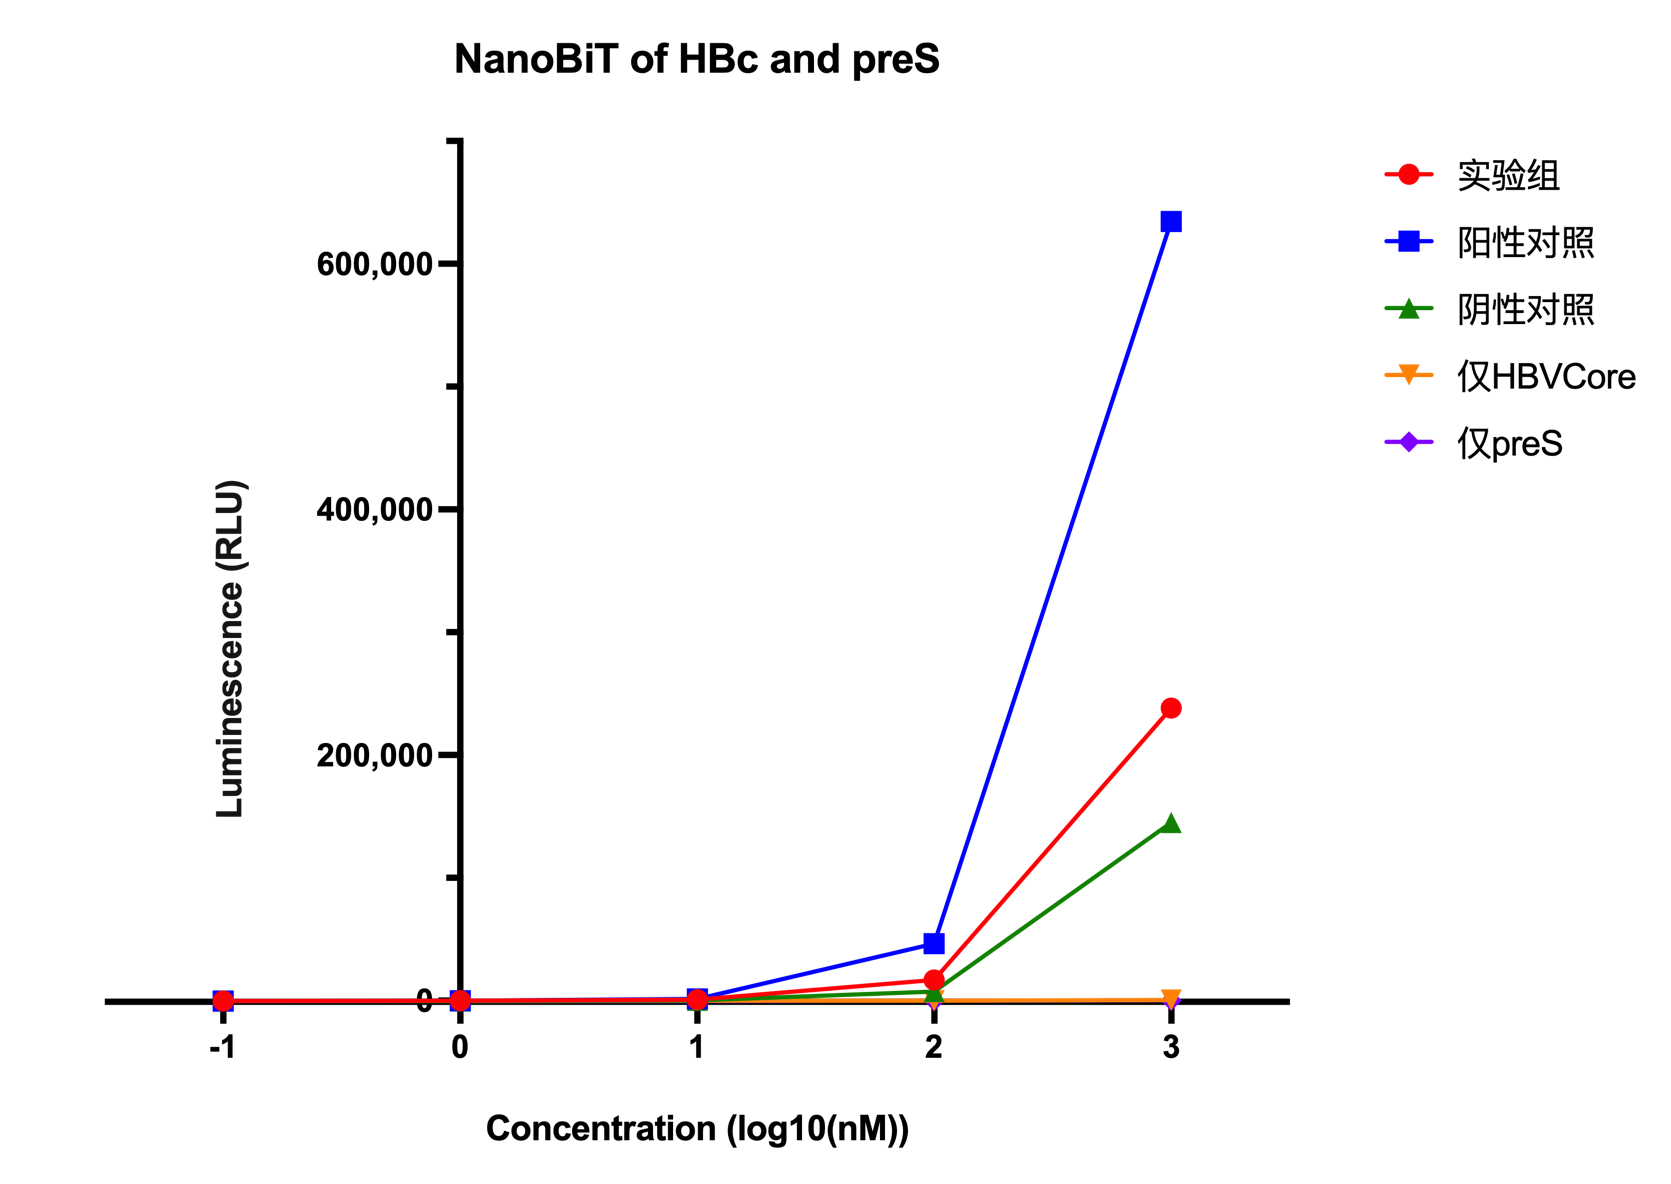
\includegraphics[width=0.62\textwidth]{figures/result/result_31.png}
  \caption{NanoBiT体系1:1浓度比例下的初步检测结果。HBVCp182-SmBiT与preS 87--114-LgBiT组合的发光信号高于阴性对照，阳性对照显示检测体系具有足够的信号上限。}
  \label{fig:nanobit-one-to-one}
\end{figure}

进一步固定HBVCp182-SmBiT浓度为50 nM并滴定含preS 87--114的LgBiT融合蛋白时，实验组与阴性对照之间的分离随LgBiT-preS浓度升高而逐渐增强。实验组总发光信号呈浓度依赖性上升，扣除背景后的特异信号呈现趋于饱和的趋势，符合有限互作复合物形成的特征。定量结果显示，当LgBiT-preS终浓度为40、80和160 nM时，实验组发光信号分别约为3295.33、4873.67和7194.67 RLU，而对应阴性对照分别约为915.67、1561.67和2697.67 RLU。相应Z-factor分别为0.608、0.695和0.623，均超过0.5；20 nM条件下Z-factor约为0.485，处于临界范围。

\begin{figure}[htbp]
  \centering
  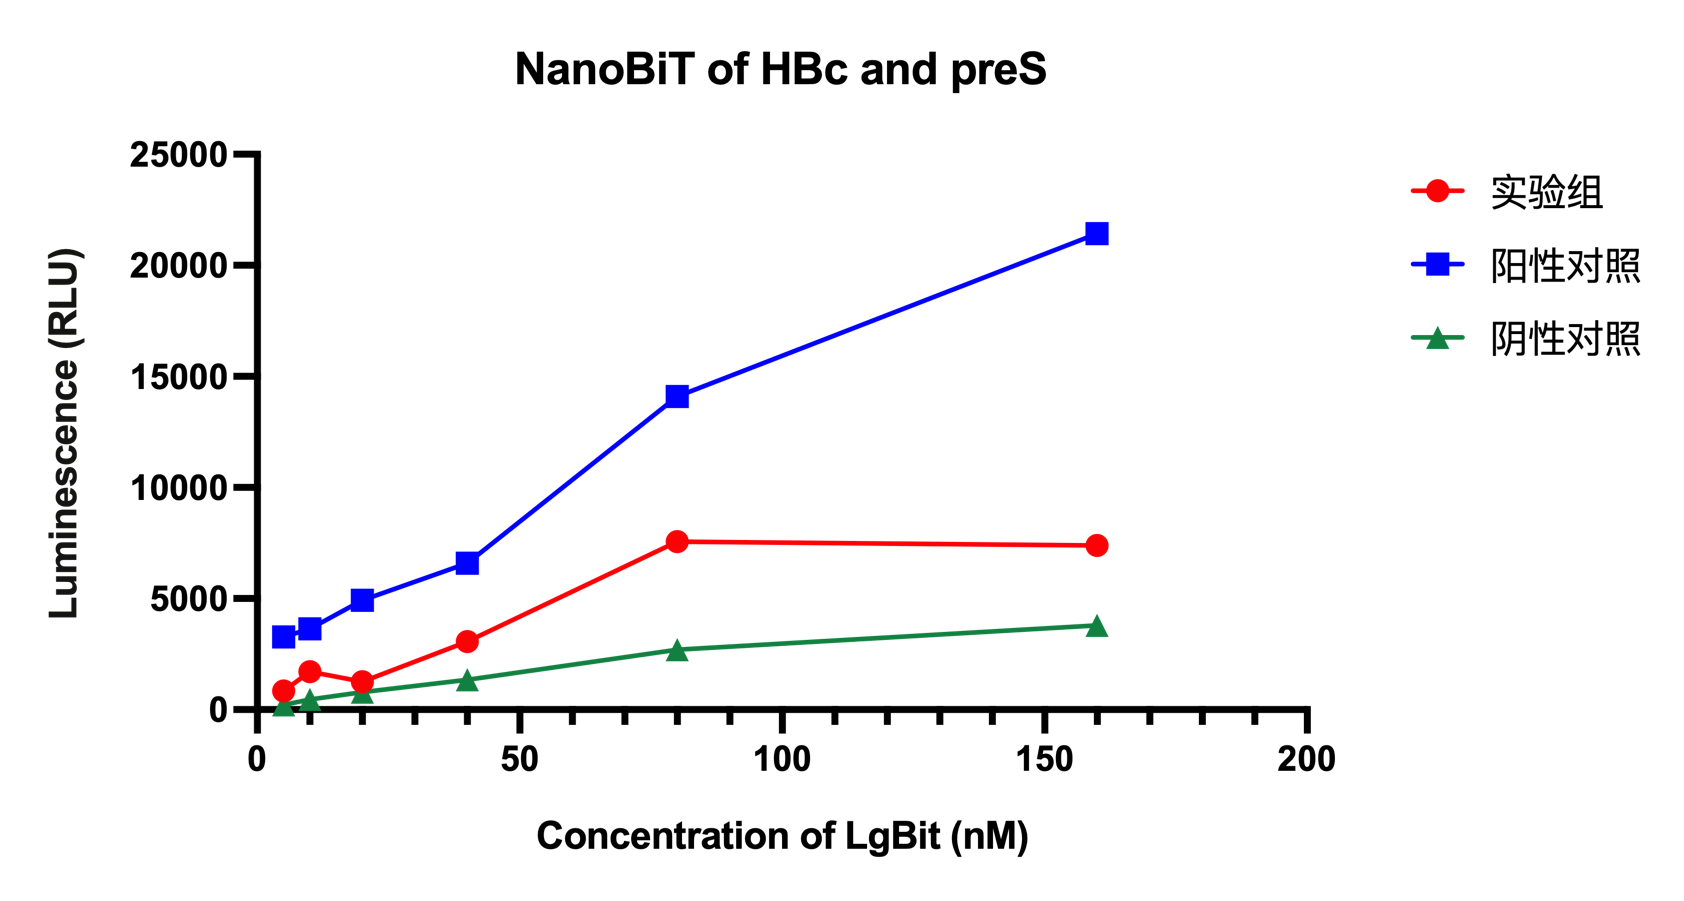
\includegraphics[width=0.46\textwidth]{figures/result/result_32.png}
  \hfill
  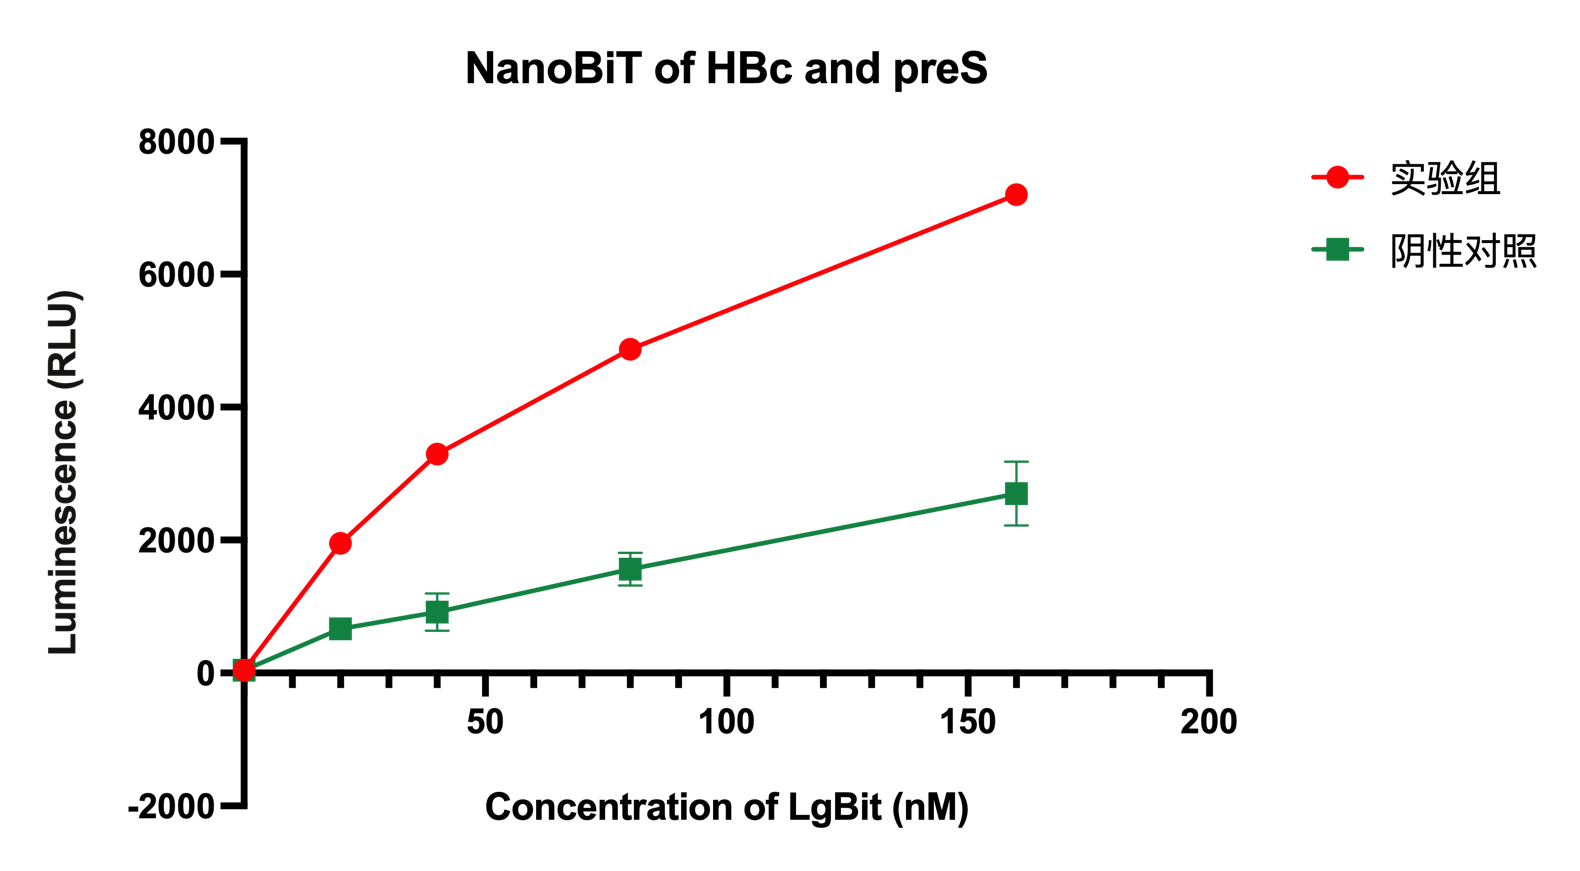
\includegraphics[width=0.46\textwidth]{figures/result/result_33.png}
  \par\medskip
  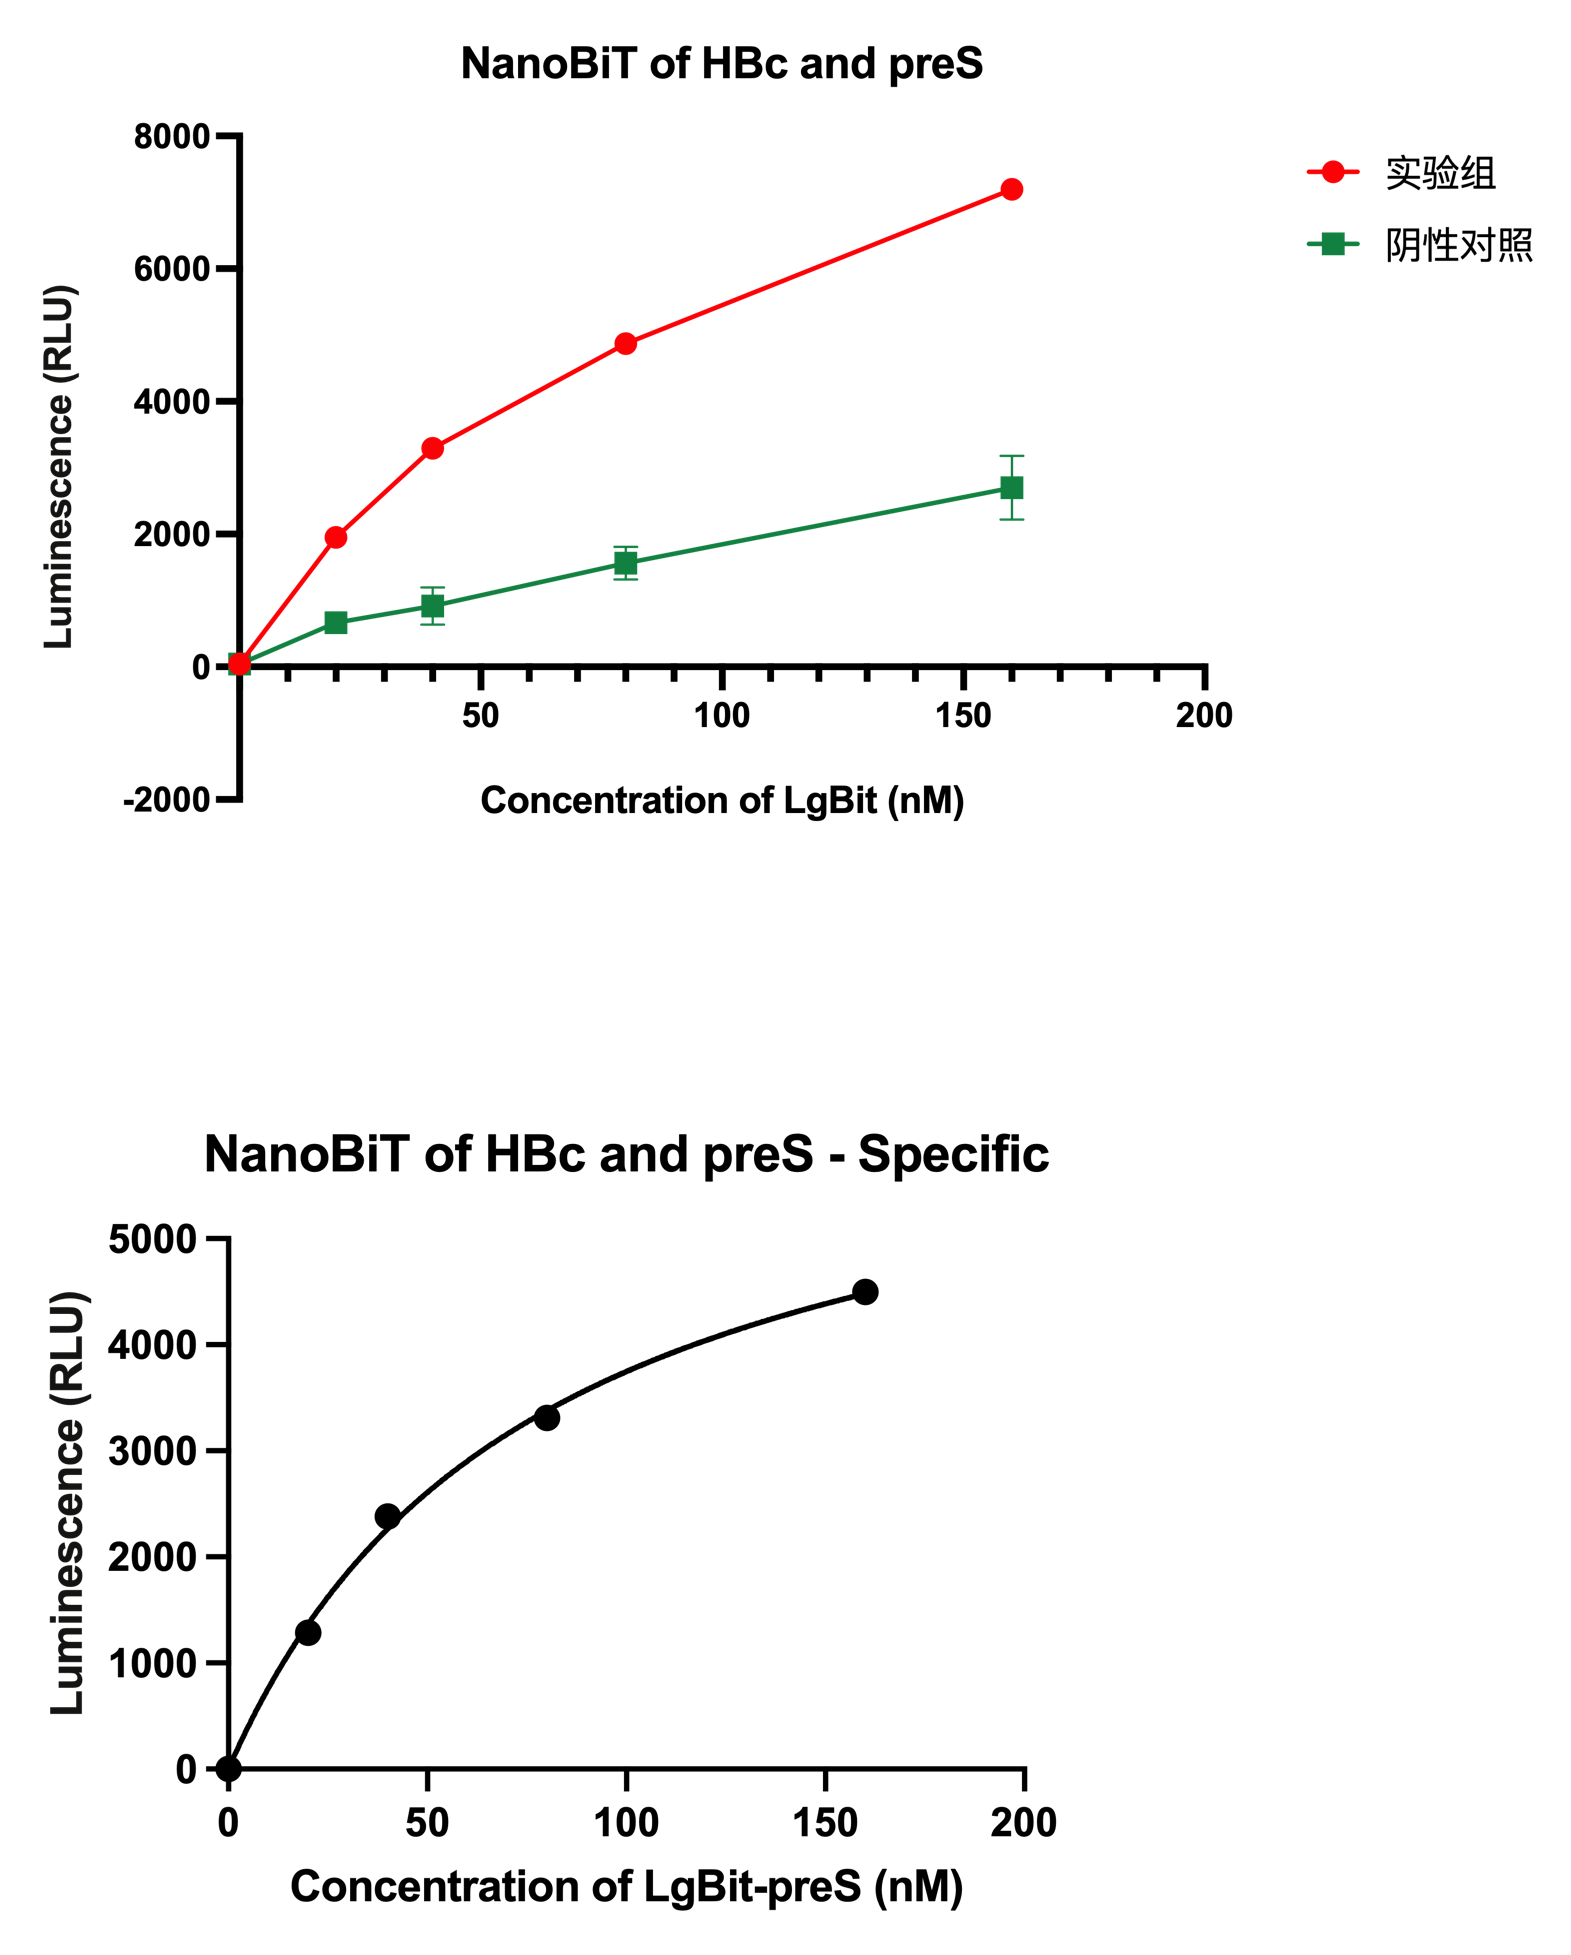
\includegraphics[width=0.35\textwidth]{figures/result/result_34.png}
  \hfill
  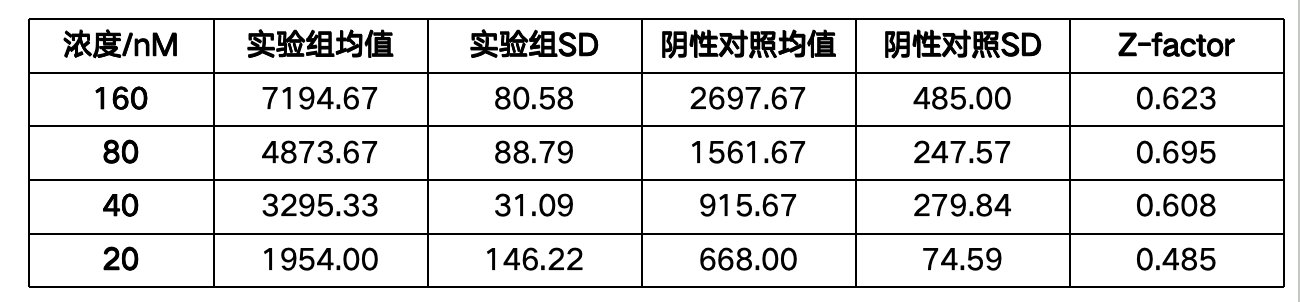
\includegraphics[width=0.55\textwidth]{figures/result/result_35.png}
  \caption{固定HBVCp182-SmBiT浓度后的NanoBiT滴定结果。随着preS 87--114-LgBiT浓度升高，实验组与阴性对照逐渐分离，部分条件下Z-factor超过0.5，显示该体系具备后续定量比较的可行性。}
  \label{fig:nanobit-fixed-core}
\end{figure}

上述结果表明，在合适蛋白浓度条件下，NanoBiT体系能够提供比ELISA更稳定的实验组--阴性对照分离度和更好的统计学窗口。尤其当LgBiT-preS浓度达到40 nM及以上时，该体系已具备进行后续定量比较的基础。结合ELISA结果，可以认为NanoBiT更适合作为本研究后续分析preS关键突变体和小分子抑制作用的主要检测平台。

\subsection{新纯化HBVCp182-SmBiT重复NanoBiT滴定实验}

使用合并后的新纯化HBVCp182-SmBiT进一步重复HBc与preS 87--114相互作用的NanoBiT浓度梯度实验。结果显示，随着GST-LgBiT-preS 87--114融合蛋白浓度升高，实验组发光信号持续增加；阴性对照虽然也随蛋白浓度升高而升高，但始终明显低于实验组。扣除阴性对照后的特异性信号呈现趋于饱和的曲线形态，说明该体系主要报告有限的HBc--preS相互作用，而不是无上限的非特异性NanoLuc片段互补。

定量结果显示，在10--640 nM LgBiT-preS范围内，实验组平均信号由939.00 RLU增加至11320.67 RLU，阴性对照由93.00 RLU增加至4691.67 RLU，特异性信号由846.00 RLU增加至6629.00 RLU。10、20、160和320 nM条件下的Z-factor均高于0.5，其中20 nM和320 nM分别达到0.859和0.770，说明这些浓度下实验组和阴性对照具有较好统计分离度。40、80和640 nM条件下Z-factor低于0.5，主要可能与实验组变异或高浓度背景升高有关。尽管80 nM条件的Z-factor为0.403，但该条件下实验组信号明显高于背景，曲线仍处于较敏感的上升区间，且蛋白消耗低于更高浓度条件，因此被选为含foldon体系下小分子初筛的工作浓度。

\begin{figure}[htbp]
  \centering
  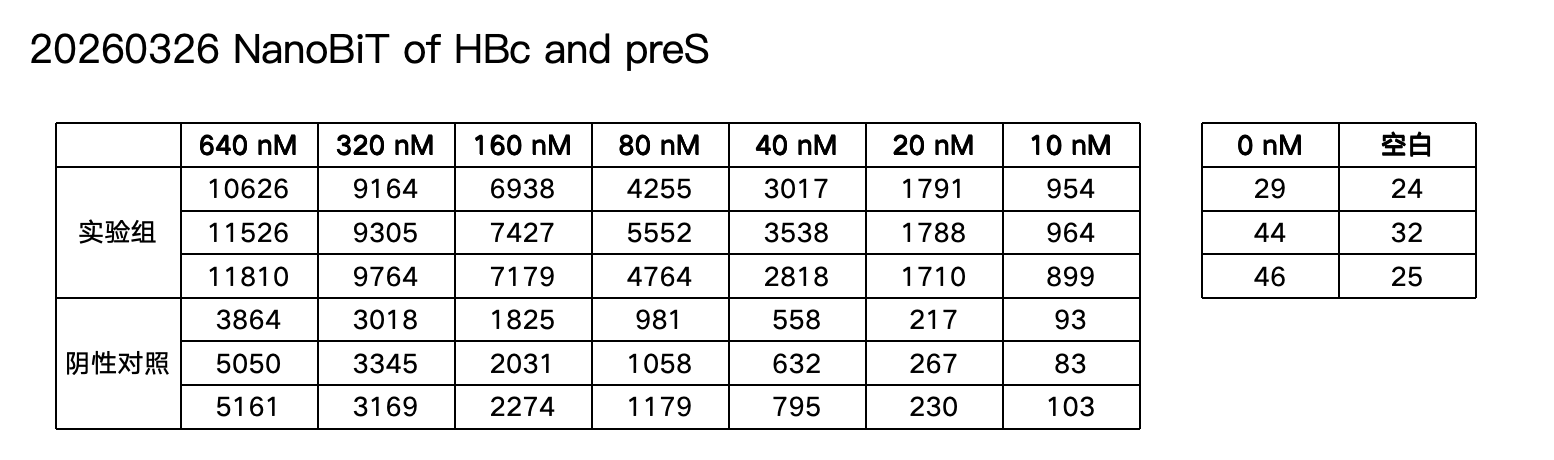
\includegraphics[width=0.82\textwidth]{figures/result/result_40.png}
  \par\medskip
  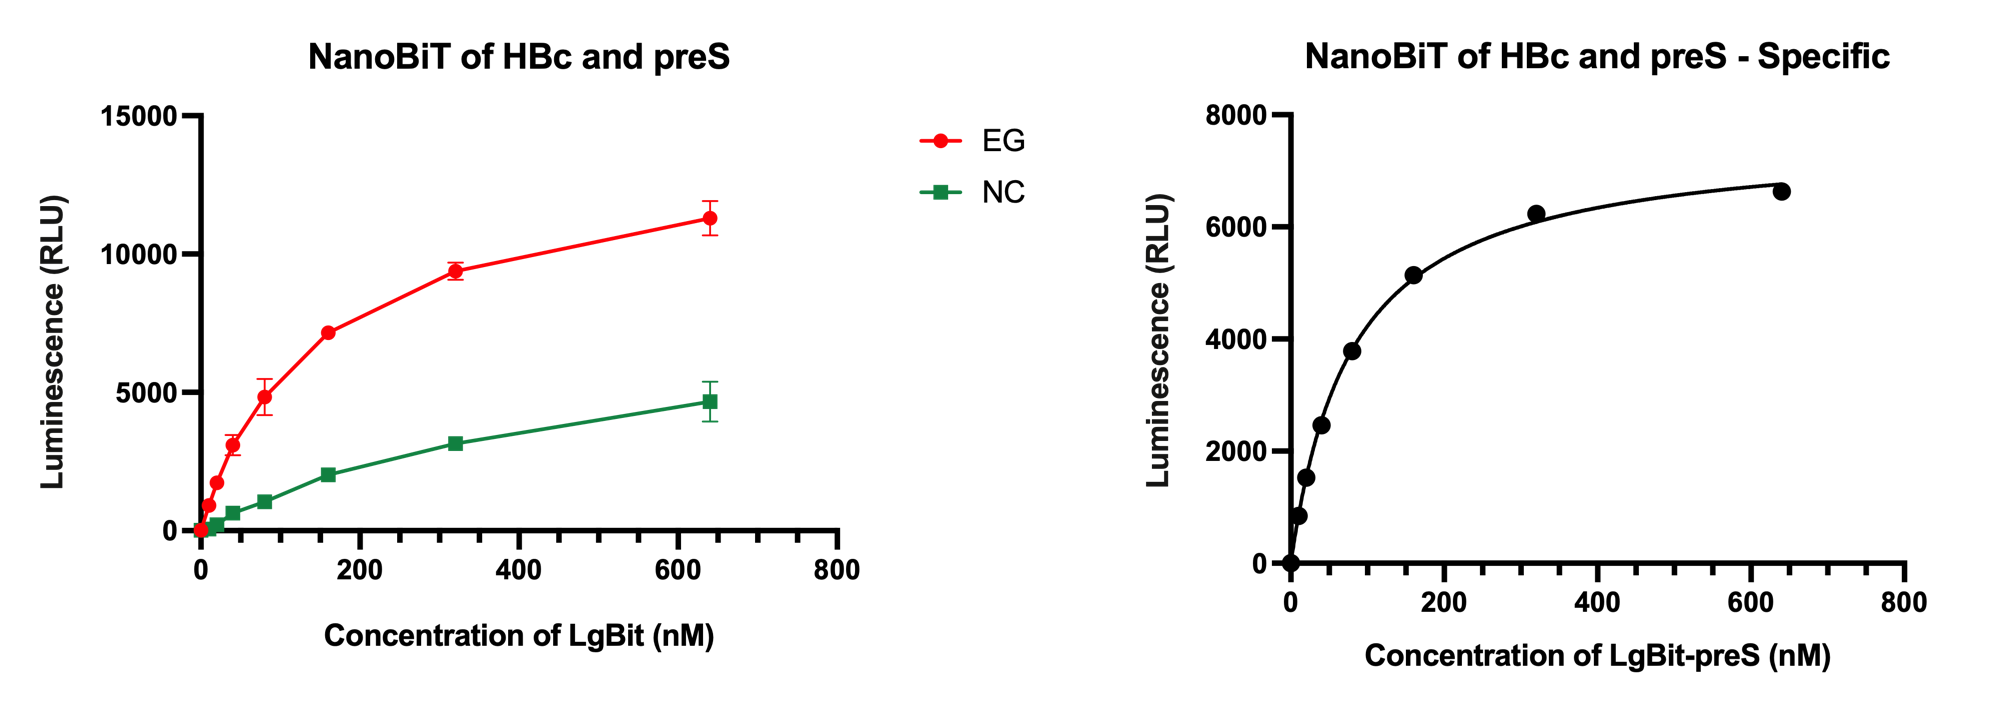
\includegraphics[width=0.52\textwidth]{figures/result/result_41.png}
  \hfill
  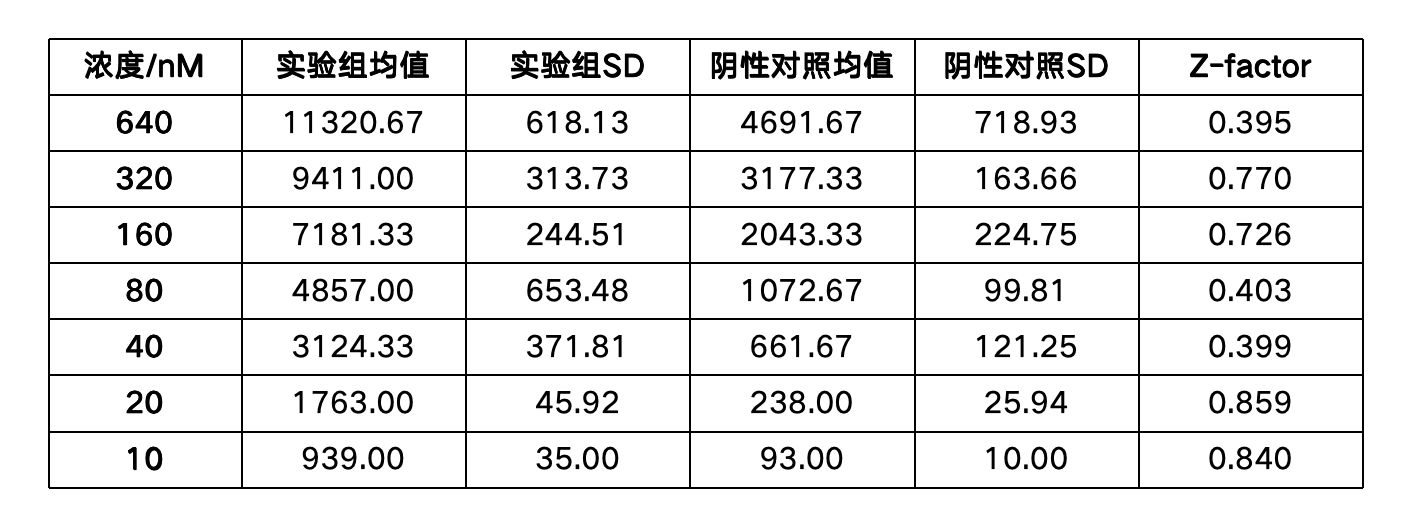
\includegraphics[width=0.38\textwidth]{figures/result/result_42.png}
  \caption{使用新纯化HBVCp182-SmBiT重复NanoBiT滴定实验。实验组信号随LgBiT-preS浓度升高而增加，扣除阴性对照后的特异性信号呈饱和趋势。}
  \label{fig:repurified-hbvcp182-nanobit-titration}
\end{figure}

\subsection{含foldon构建体条件下的小分子抑制实验}

在上述滴定结果基础上，首先使用含foldon的LgBiT-preS体系检测候选小分子对HBc--preS相互作用的影响。初筛中比较了Triton X-100、NP-40和香叶醇对NanoBiT发光信号的影响。直接加入小分子时，三种小分子均未产生充分清晰的抑制窗口。Triton X-100和NP-40的实验组信号在高浓度区间有一定下降，但阴性对照也发生轻度变化；香叶醇处理下的特异性信号波动更明显，整体趋势不够稳定。

这一结果提示，在直接加药条件下，小分子对HBc--preS相互作用的抑制不易被稳定观察。可能原因包括候选小分子与HBVCp182-SmBiT接触时间不足、检测浓度范围尚未覆盖有效区间，以及含foldon的LgBiT-preS构建体可能以多价形式增强表观结合，从而降低小分子竞争效应的可观察性。

\begin{figure}[htbp]
  \centering
  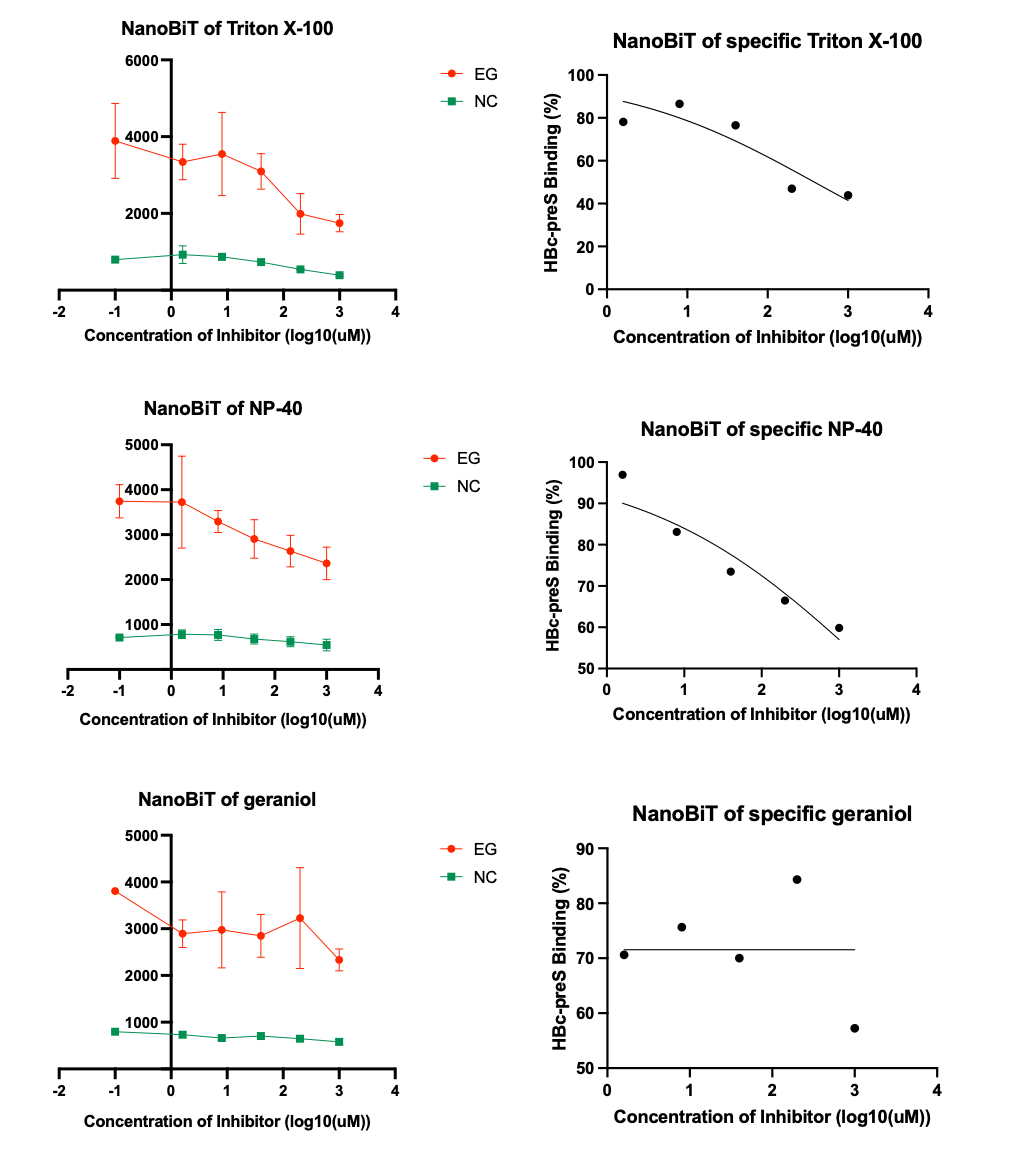
\includegraphics[width=0.70\textwidth]{figures/result/result_43.png}
  \caption{含foldon构建体条件下的小分子抑制初筛。直接加入Triton X-100、NP-40和香叶醇时，HBc--preS特异性信号未形成稳定清晰的剂量依赖性抑制窗口。}
  \label{fig:foldon-inhibitor-initial}
\end{figure}

为增强小分子与HBVCp182-SmBiT的接触，后续实验改为先将候选小分子与HBVCp182-SmBiT预先孵育，再加入LgBiT-preS或LgBiT阴性对照进行检测，并提高抑制剂浓度范围。在该条件下，Triton X-100、NP-40和香叶醇对HBc--preS发光信号的抑制趋势更加明显，尤其在高浓度区间，实验组信号出现更大幅度下降，扣除阴性对照后的相对结合百分比也呈下降趋势。

尽管如此，含foldon体系仍不适合直接计算准确的表观亲和力或IC$_{50}$。当前使用的GST-LgBiT-preS 87--114-foldon构建体含有foldon结构域，可能诱导三聚化并增强多价结合；同时GST标签本身也具有二聚化倾向。这些因素可能提高体系的表观亲和力和发光信号，使小分子抑制被部分掩盖，也使剂量--反应曲线不能直接反映单价HBc--preS相互作用。因此，后续实验进一步转向不含foldon的LgBiT构建体，并尝试降低GST标签二聚化带来的影响。

\begin{figure}[htbp]
  \centering
  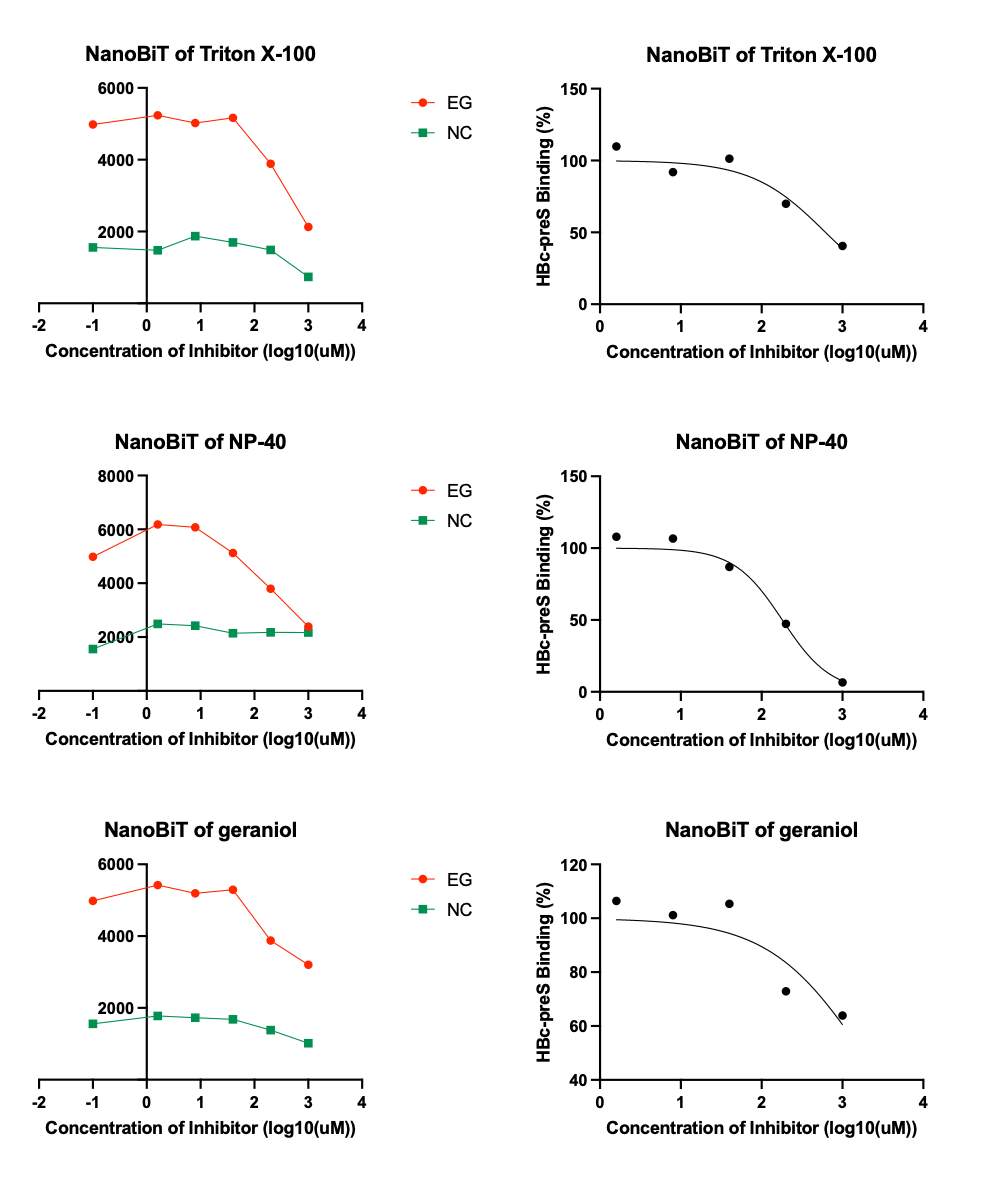
\includegraphics[width=0.70\textwidth]{figures/result/result_44.png}
  \caption{预孵育并提高小分子浓度后的含foldon体系抑制实验。高浓度区间实验组信号和相对结合百分比下降更明显，但foldon和GST相关多价效应限制了定量解释。}
  \label{fig:foldon-inhibitor-preincubation}
\end{figure}

\subsection{不含foldon的LgBiT构建体制备与NanoBiT滴定}

为降低foldon介导的多聚化效应，进一步制备了不含foldon的GST-LgBiT-preS 87--114-His和GST-LgBiT-His构建体。GST亲和纯化结果显示，GST-LgBiT-preS 87--114-His可在GST柱洗脱组分中观察到较清晰的目标条带，说明该构建体能够被GST柱有效捕获并洗脱。相比之下，GST-LgBiT-His在GST柱洗脱组分中回收较少，而流穿液中仍可见目标大小附近条带，提示该蛋白在当前条件下不易通过GST柱充分回收。

为提高阴性对照蛋白产量，进一步从GST柱流穿液出发，通过His标签富集和Q HP柱纯化获得GST-LgBiT-His。Q柱图谱中约16.03 mL处出现明显主峰，SDS-PAGE显示16--22管附近存在较集中的GST-LgBiT-His条带，说明补充纯化策略可获得足够的阴性对照蛋白用于后续实验。

\begin{figure}[htbp]
  \centering
  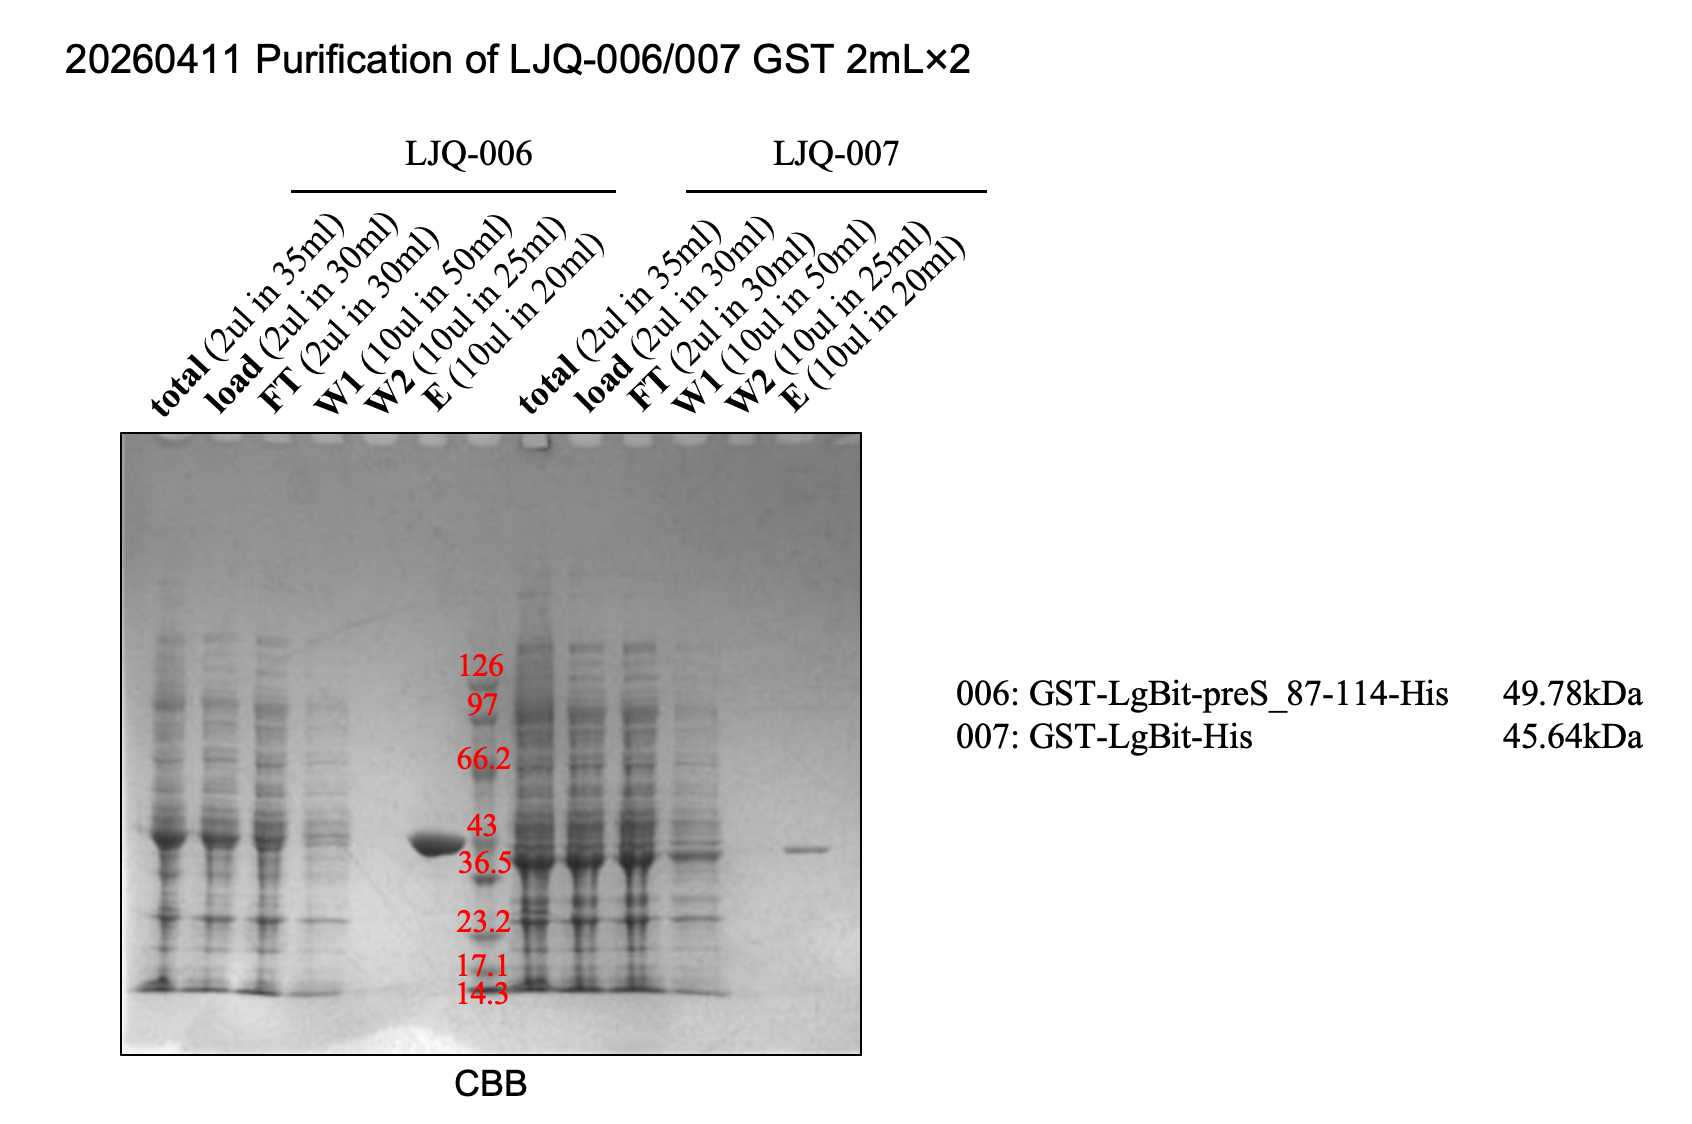
\includegraphics[width=0.58\textwidth]{figures/result/result_45.png}
  \caption{不含foldon的GST-LgBiT-preS 87--114-His和GST-LgBiT-His的GST柱纯化结果。GST-LgBiT-preS 87--114-His在洗脱组分中较为明显，而GST-LgBiT-His回收效率较低。}
  \label{fig:foldon-free-gst-purification}
\end{figure}

\begin{figure}[htbp]
  \centering
  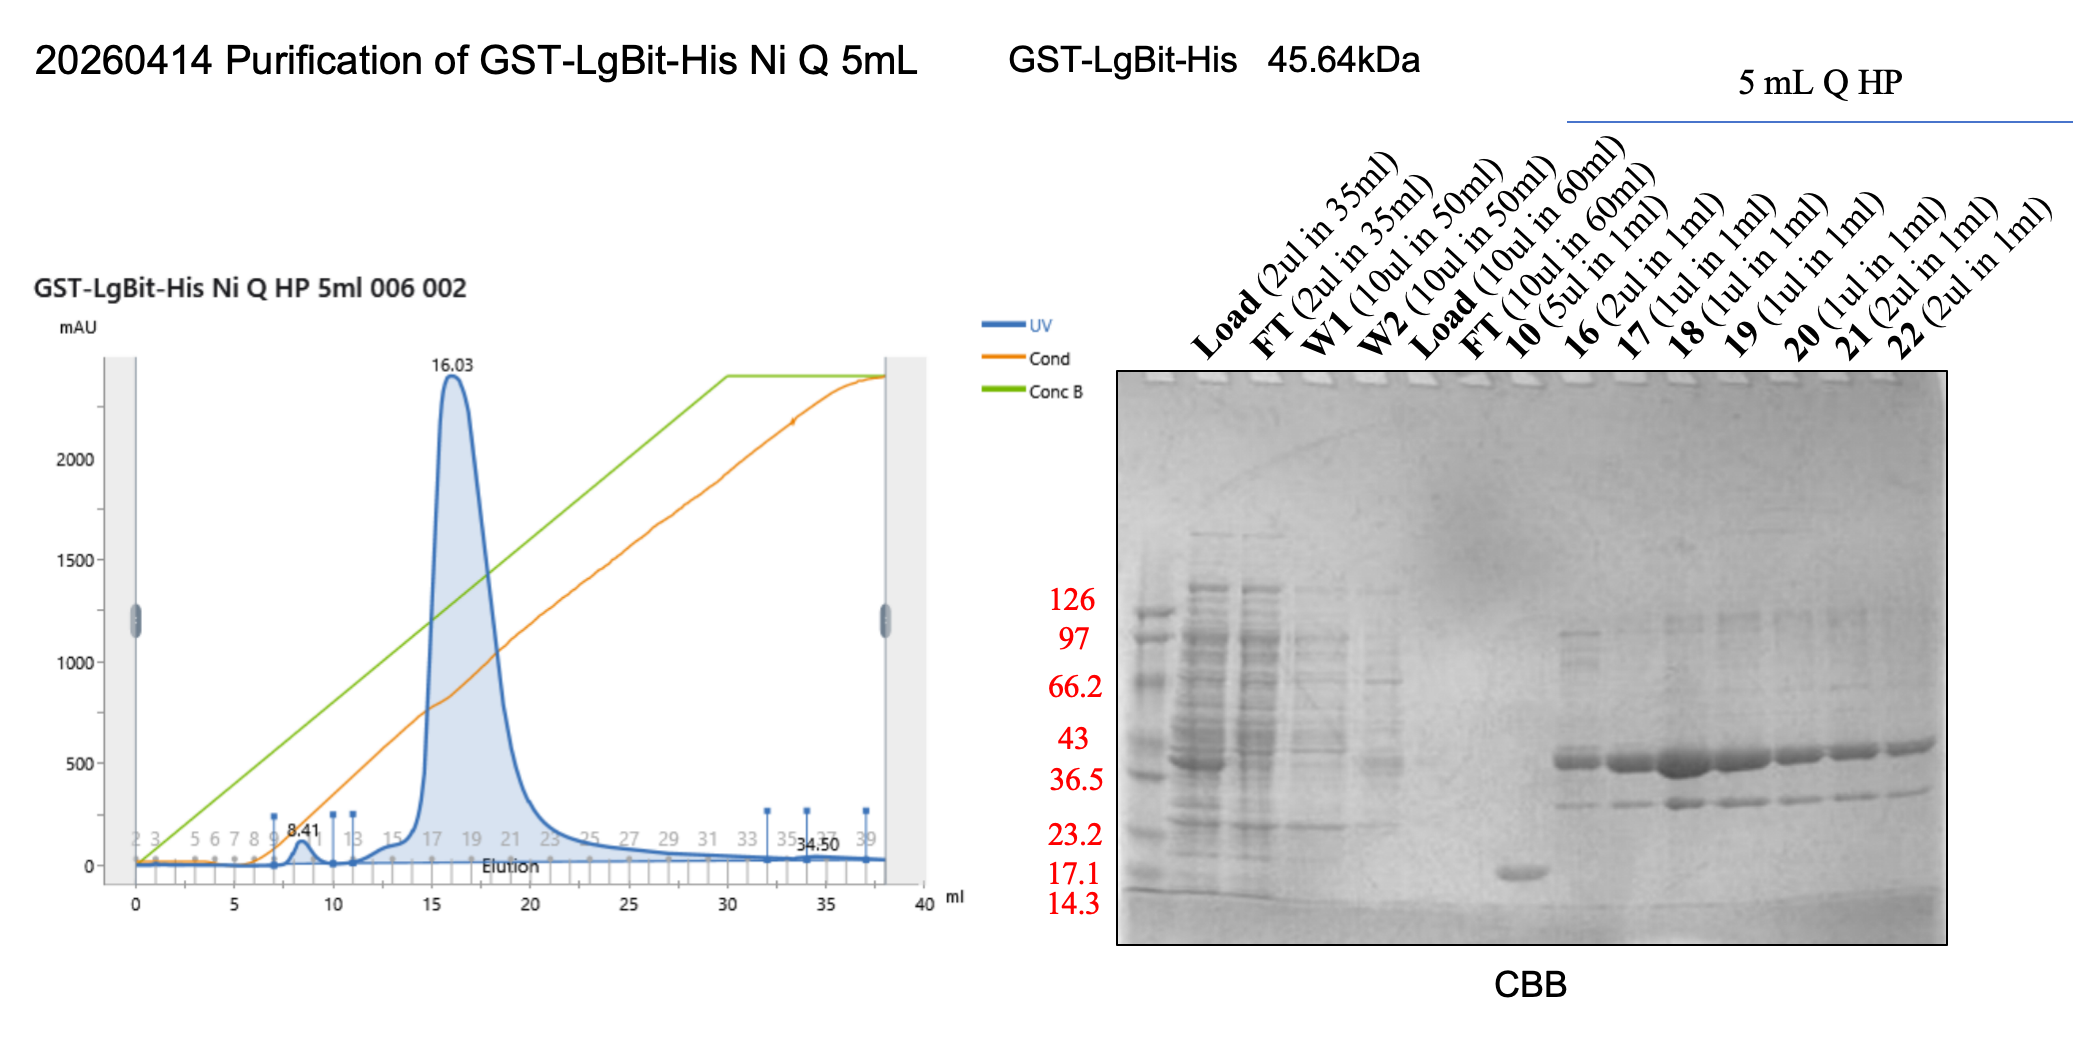
\includegraphics[width=0.82\textwidth]{figures/result/result_46.png}
  \caption{GST-LgBiT-His从GST柱流穿液出发的进一步纯化。Ni柱富集和Q HP柱纯化后，可获得用于后续NanoBiT检测的阴性对照蛋白。}
  \label{fig:gst-lgbit-his-further-purification}
\end{figure}

使用新纯化的不含foldon构建体重复HBc--preS NanoBiT滴定实验。与含foldon体系相比，不含foldon的LgBiT-preS不再具有三聚化带来的多价优势，因此需要更高浓度才能产生足够的特异性发光信号。实验组信号随着LgBiT-preS浓度增加而持续上升，阴性对照维持在较低水平但仍具有一定浓度依赖背景。扣除阴性对照后，特异性信号逐渐升高并呈现弯曲趋势，说明该体系仍可检测HBc--preS相互作用，但表观结合强度低于含foldon体系。

根据不同浓度范围的滴定结果，后续小分子抑制实验选择1000 nM LgBiT作为工作浓度。该浓度能够提供清楚的实验组与阴性对照分离，同时保留可观察的抑制空间；若浓度过低，信号窗口不足，而浓度过高则可能增加背景并削弱抑制剂引起的相对变化。

\begin{figure}[htbp]
  \centering
  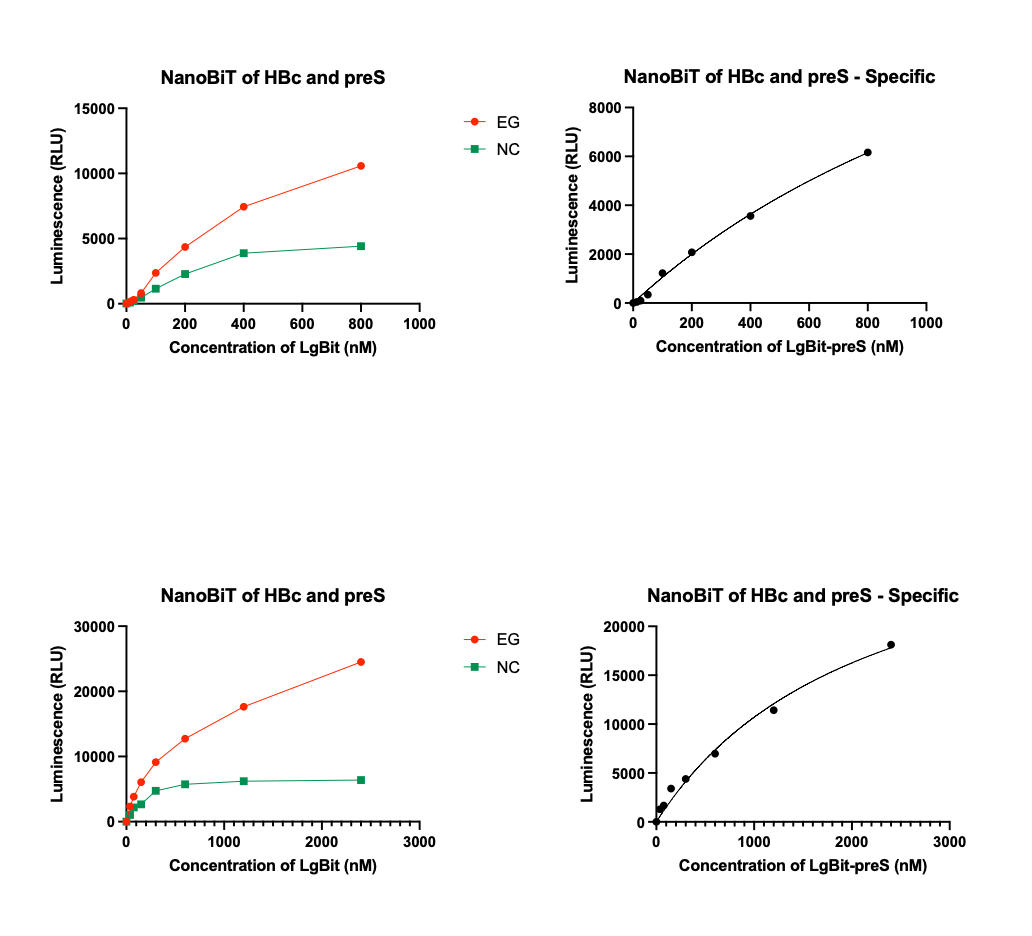
\includegraphics[width=0.76\textwidth]{figures/result/result_47.png}
  \caption{不含foldon体系下的HBc--preS NanoBiT滴定结果。实验组信号随LgBiT-preS浓度升高而增加，提示该体系可用于后续小分子抑制检测。}
  \label{fig:foldon-free-nanobit-titration}
\end{figure}

\subsection{不含foldon体系下的小分子抑制结果与GST标签影响}

在不含foldon体系中重新检测Triton X-100、NP-40和香叶醇对HBc--preS结合的影响。结果显示，三种小分子在高浓度区间均使实验组发光信号下降，其中Triton X-100和香叶醇的高浓度抑制趋势较为明显，NP-40的抑制曲线相对平缓且波动较大。扣除阴性对照后，Triton X-100和香叶醇的特异性结合百分比下降更清楚，说明不含foldon体系较含foldon体系更容易显示小分子作用。

需要注意的是，高浓度小分子存在时，阴性对照信号也发生改变，提示这些分子可能不仅影响HBc--preS结合，也可能影响蛋白稳定性、NanoLuc片段互补效率或检测体系背景。因此，在目前数据基础上不宜直接给出IC$_{50}$。后续若进行定量拟合，需要加入NanoBiT片段互补本身的控制、蛋白聚集或变性控制，以及多次独立重复，并在背景受控的浓度区间内进行分析。

\begin{figure}[htbp]
  \centering
  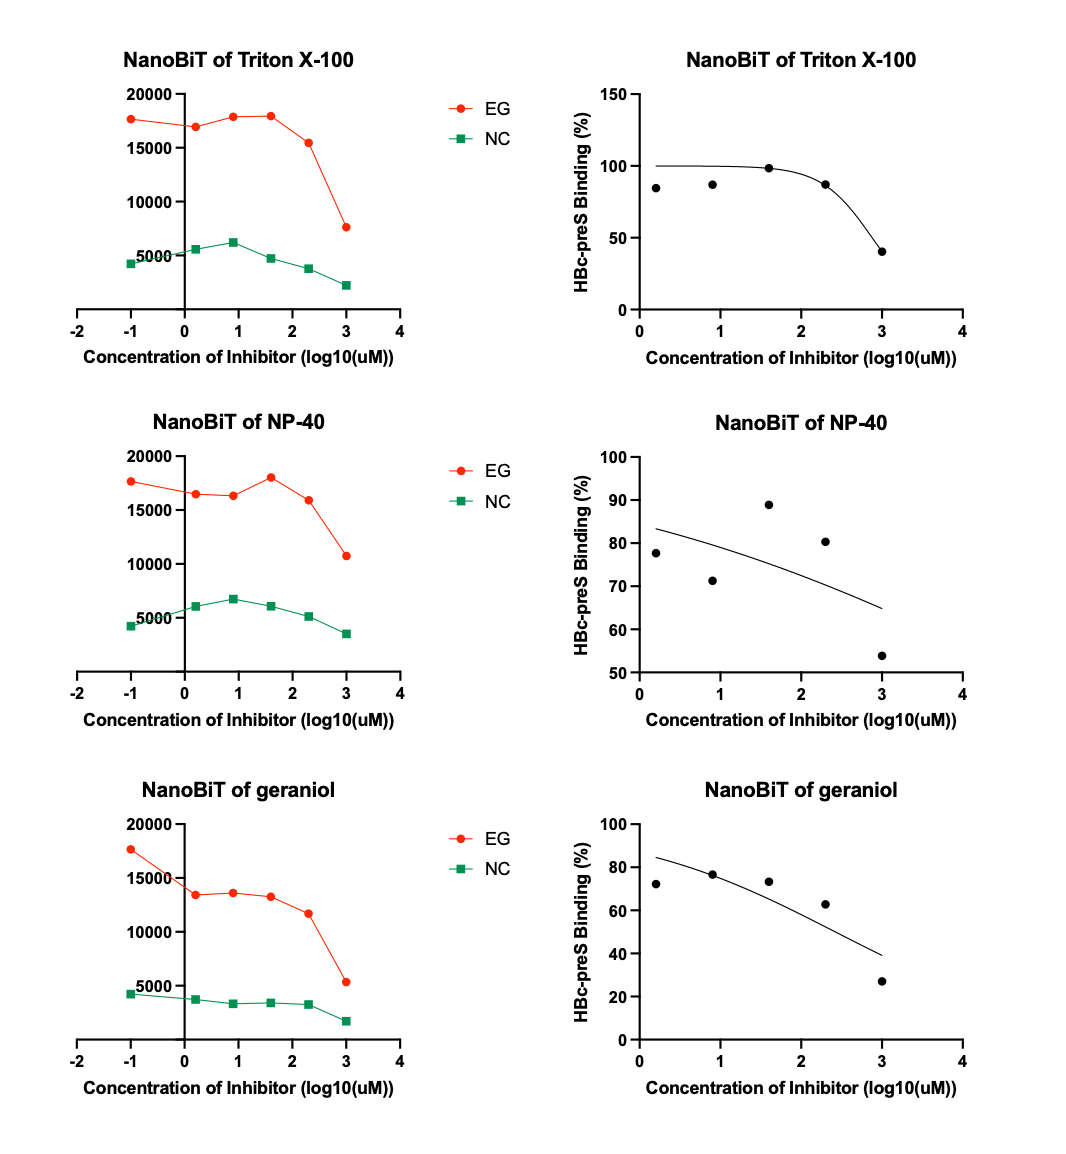
\includegraphics[width=0.74\textwidth]{figures/result/result_48.png}
  \caption{不含foldon体系下的小分子抑制实验。Triton X-100和香叶醇在高浓度区间显示更明显的相对抑制趋势，但阴性对照背景变化提示仍需进一步控制体系背景。}
  \label{fig:foldon-free-inhibitor-assay}
\end{figure}

由于GST标签本身可形成二聚体，可能使LgBiT-preS或LgBiT阴性对照发生非目标性聚集，从而影响NanoBiT信号解释，因此进一步使用PPase去除GST标签。SDS-PAGE结果显示，酶切后样品中出现与GST、LgBiT-preS和LgBiT相对应的条带；与未酶切样品相比，目标融合蛋白发生明显迁移变化，说明GST标签去除基本成功。该步骤为后续更接近单体状态的preS突变体比较提供了必要条件。

\begin{figure}[htbp]
  \centering
  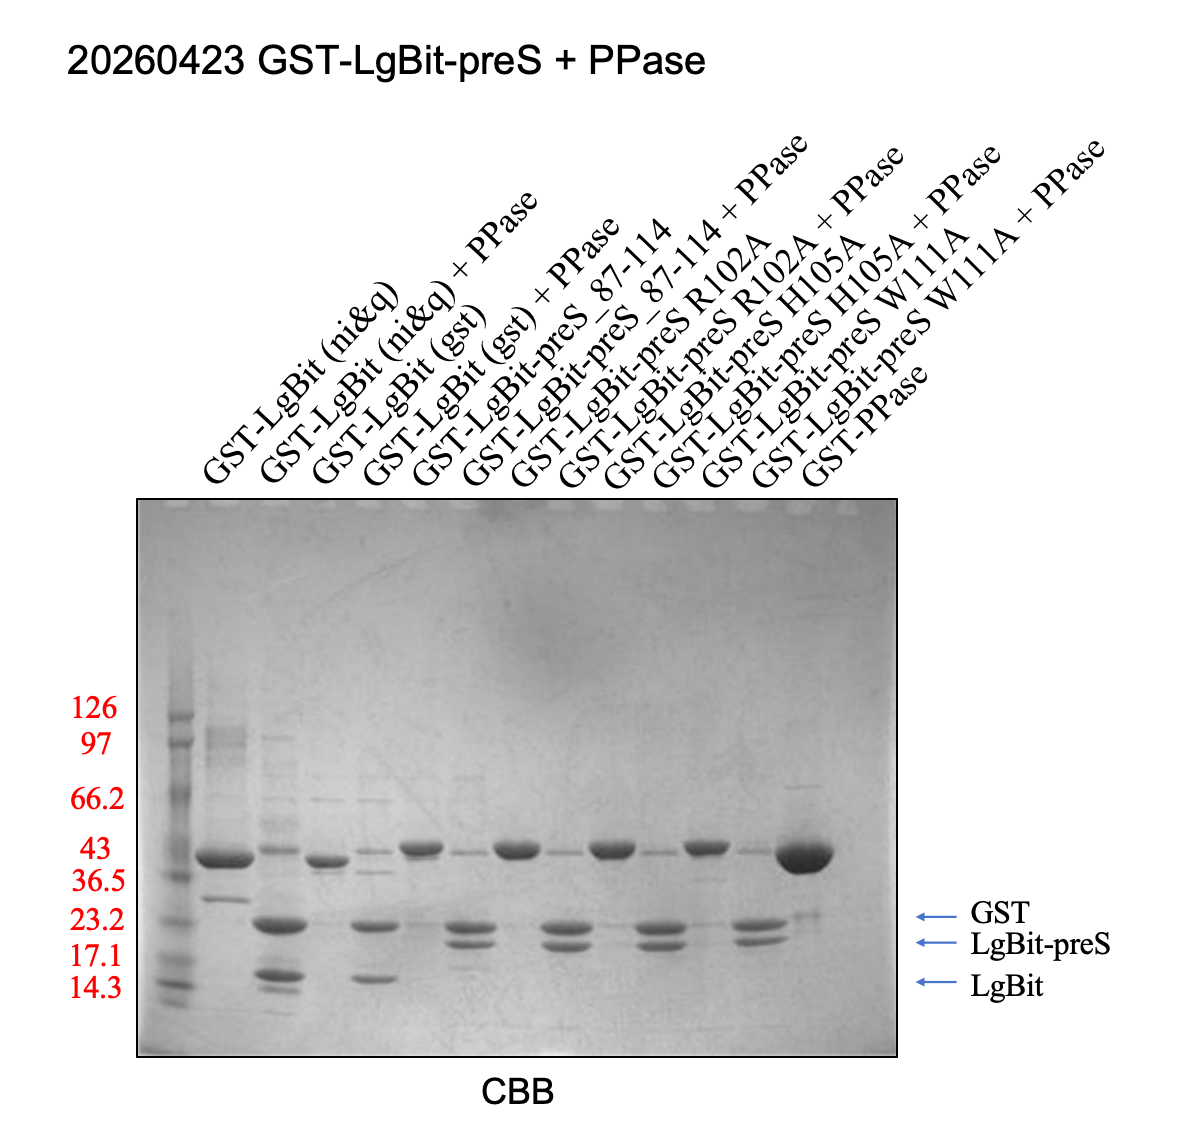
\includegraphics[width=0.58\textwidth]{figures/result/result_49.png}
  \caption{PPase切除GST标签的SDS-PAGE分析。酶切后可观察到GST、LgBiT-preS和LgBiT相关条带，提示GST标签去除基本成功。}
  \label{fig:ppase-gst-cleavage}
\end{figure}

\subsection{去除GST标签后preS突变体与HBc结合能力比较}

最后，利用酶切后的LgBiT-preS蛋白比较wild-type preS 87--114及R102A、H105A和W111A突变体与HBVCp182-SmBiT的结合能力。结果显示，wild-type preS 87--114在整个LgBiT浓度范围内均产生最高发光信号，且随浓度升高持续增加。相比之下，三个突变体的信号均显著降低，并接近或仅略高于LgBiT阴性对照。

从趋势上看，R102A和H105A的结合信号下降最明显，整体接近阴性对照水平；W111A仍保留一定残余信号，但明显低于wild-type preS 87--114。该结果表明R102、H105和W111均参与preS 87--114与HBc的结合界面，其中R102和H105对结合贡献尤其明显。更重要的是，该实验说明经过foldon去除和GST酶切后的NanoBiT体系能够区分不同preS突变体的结合能力，具有用于机制分析和后续突变筛选的可行性。

\begin{figure}[htbp]
  \centering
  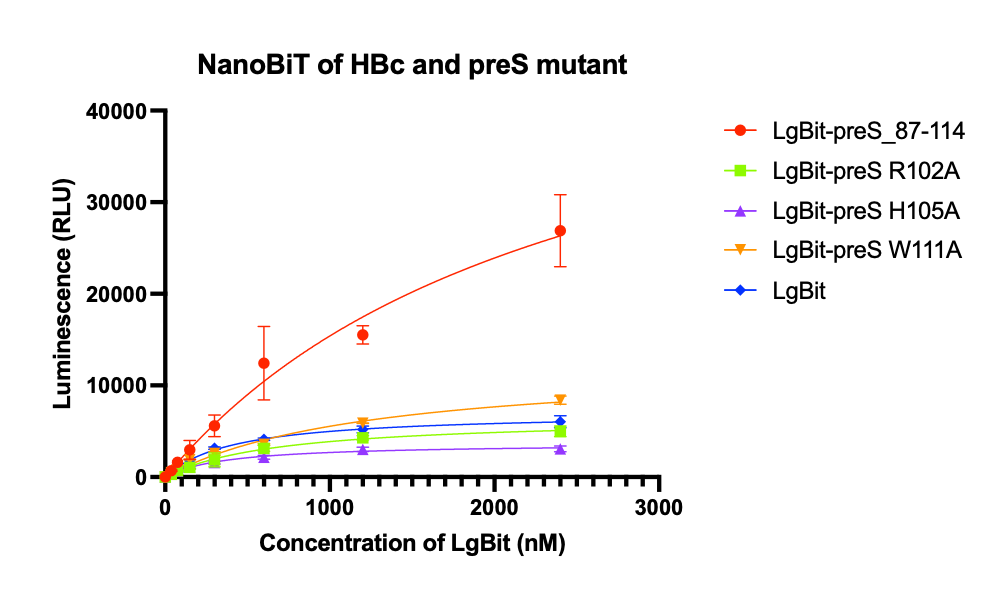
\includegraphics[width=0.56\textwidth]{figures/result/result_50.png}
  \hfill
  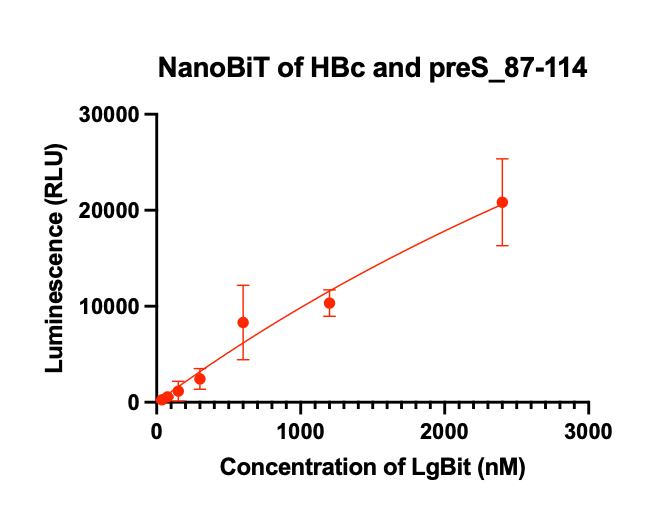
\includegraphics[width=0.36\textwidth]{figures/result/result_51.png}
  \caption{去除GST标签后wild-type preS 87--114与preS突变体的NanoBiT比较。R102A、H105A和W111A均显著降低HBc--preS互作信号，其中R102A和H105A下降最明显。}
  \label{fig:pres-mutant-nanobit}
\end{figure}

\section{本章结果小结}

\subsection{ELISA体系的主要结论}

本章首先建立并比较了HBc--preS体外互作检测体系。三种ELISA构型分别从HBc直接包被、StrepXT捕获preS和抗core Fab捕获HBc三个角度优化检测流程，但均受到非特异背景高、信号窗口窄或重复性不足的限制，难以作为后续突变体比较和小分子抑制评价的主要平台。相比之下，NanoBiT体系能够在较少洗涤干扰的条件下检测HBVCp182与preS 87--114之间的相互作用，并在合适浓度下获得较好的实验组--阴性对照分离。

\subsection{NanoBiT平台的优化结论}

后续实验进一步优化了NanoBiT平台。重新纯化HBVCp182-SmBiT提高了体系稳定性；含foldon体系可检测HBc--preS相互作用并初步观察小分子抑制趋势，但foldon和GST带来的多价效应限制了定量解释；不含foldon并进一步去除GST标签的体系更适合分析单价preS片段与HBc的相互作用。

\subsection{preS关键残基验证与平台意义}

基于该优化体系，preS R102A、H105A和W111A突变均显著降低HBc--preS互作信号，支持这些残基在结构界面中的关键作用。整体来看，本研究已建立可用于机制验证和候选小分子初步评价的非感染性体外NanoBiT平台，为后续围绕HBc--preS界面的抗病毒策略研究提供了实验基础。

\chapter{总结与展望}

\section{研究总结}

HBV感染性病毒颗粒的形成依赖成熟核衣壳与包膜蛋白之间的特异性识别，其中L-HBsAg preS区域与HBc核衣壳的相互作用是病毒包膜化过程中的关键环节。近期结构研究提出preS 87--114片段可作为基质样结构域识别HBc表面沟槽，并指出R102、H105和W111等残基可能参与关键界面形成，同时W111插入的HBc疏水口袋具有被小分子竞争占据的潜力。本研究围绕这一结构模型，建立非感染性重组蛋白体外检测体系，用于定量验证HBc--preS相互作用及其受突变体和小分子影响的规律。

本研究首先比较了三种ELISA构型，包括HBc直接包被、StrepXT捕获preS以及抗core Fab捕获HBc。结果显示，不同构型虽然分别改善了核心蛋白或preS的呈递方式，但均受到非特异背景、固相吸附、洗涤导致弱相互作用解离以及统计窗口不足等限制，难以作为后续系统筛选和定量比较的主要平台。该结果提示HBc--preS相互作用更适合在减少洗涤和固定化干扰的体系中检测。

在此基础上，本研究建立了NanoBiT发光互补体系，将SmBiT融合至HBVCp182，将LgBiT融合至preS 87--114片段或相应阴性对照。初步实验表明，HBVCp182-SmBiT与LgBiT-preS组合能够产生高于阴性对照的发光信号；固定HBVCp182-SmBiT并滴定LgBiT-preS后，实验组与阴性对照之间出现可量化分离，部分条件下Z-factor超过0.5，说明该体系能够报告HBc--preS相互作用并具备进一步优化空间。后续通过重新纯化HBVCp182-SmBiT、比较Q柱合并组分活性以及优化LgBiT构建体，进一步提高了实验体系的可用性。

小分子抑制实验表明，在含foldon体系中，Triton X-100、NP-40和香叶醇直接加入时抑制趋势不够稳定；经预孵育并提高小分子浓度后，高浓度区间可观察到更明显的发光信号下降。然而foldon三聚化和GST二聚化可能增强表观结合，限制剂量--反应曲线的定量解释。进一步去除foldon后，Triton X-100和香叶醇在高浓度区间表现出更清楚的相对抑制趋势，但高浓度小分子对阴性对照信号的影响提示仍需加入更多背景控制。最后，在去除GST标签后的体系中，preS R102A、H105A和W111A突变均显著降低HBc--preS互作信号，其中R102A和H105A下降最明显，支持这些残基在HBc识别界面中的关键作用。

\section{主要结论}

本研究得到以下主要结论。第一，HBc--preS相互作用在常规固相ELISA体系中难以获得稳定、低背景且具有足够统计窗口的读数，说明该相互作用可能具有弱亲和力、构象敏感和多价依赖等特点。第二，NanoBiT体系比ELISA更适合本课题的体外定量检测需求，能够在接近溶液状态的条件下将HBVCp182与preS 87--114之间的接近事件转化为可检测发光信号。第三，HBVCp182-SmBiT的纯度和LgBiT-preS构建体的多聚化状态会显著影响检测窗口和定量解释，因此蛋白质量控制、foldon去除和GST标签影响评估是平台优化中的关键步骤。第四，preS R102、H105和W111对HBc--preS结合具有重要贡献，实验结果与结构模型中这些残基参与静电作用、氢键或疏水嵌合的解释相一致。第五，部分小分子在优化后的NanoBiT体系中可降低HBc--preS相关发光信号，提示HBc疏水口袋具有被小分子干预的可能性，但目前数据仍不足以直接给出精确IC$_{50}$或结合常数。

\section{不足与展望}

尽管本研究已经建立了可用于机制验证的体外NanoBiT平台，仍存在若干需要进一步改进的方面。首先，当前实验主要基于阶段性重复和有限批次蛋白样品，后续需要增加独立蛋白批次和独立实验重复，以更严格地评估平台稳定性、Z-factor范围和不同构建体之间的可比性。其次，小分子抑制实验中高浓度条件可能同时影响蛋白稳定性、NanoLuc片段互补效率或体系背景，因此需要加入更完整的控制组，例如仅检测NanoBiT片段互补本身、小分子对底物发光体系的影响、蛋白聚集或变性控制等。只有在背景变化可控的浓度范围内，才适合进一步进行剂量--反应拟合和IC$_{50}$估算。

其次，preS突变体分析目前集中于R102A、H105A和W111A三个关键位点。后续可以扩展至P100、L101、S113以及HBc侧对应界面残基，从preS和HBc两个方向系统验证结构模型。若能够结合更多点突变、组合突变和互补突变实验，将有助于区分静电作用、疏水嵌合和氢键网络对整体结合的相对贡献。对于小分子研究，也可在Triton X-100和香叶醇等初步候选分子的基础上，选择结构更明确、药物样性质更好的化合物进行验证，并结合计算对接或结构类似物比较，寻找更适合后续优化的分子骨架。

最后，本研究聚焦于非感染性重组蛋白体外体系，适合在较高安全性和可控性条件下解析HBc--preS相互作用本身。后续若要进一步评价该界面对HBV生命周期的影响，需要在符合生物安全规范和实验室审批要求的前提下，选择更接近细胞内环境的验证体系，例如非感染性共表达、蛋白共定位或病毒样颗粒相关模型。通过将体外定量结果、结构模型和更复杂体系中的功能验证相结合，可以更全面地评估HBc--preS界面作为新型抗HBV药物靶点的可行性。


%---------------------------------------------------------------------
%	参考文献
%---------------------------------------------------------------------

% 生成参考文献页
\printbibliography

%---------------------------------------------------------------------
%	致谢
%---------------------------------------------------------------------

\begin{acknowledgement}
  感谢陈雷教授和董咸池教授在课题设计、实验推进和论文写作过程中给予的指导。感谢课题组老师和同学在蛋白纯化、实验讨论和论文修改中提出的建议。也感谢家人和朋友在本科阶段给予的理解和支持。
\end{acknowledgement}

%---------------------------------------------------------------------
%	学术简历
%---------------------------------------------------------------------

% 详见手册中“成果列表”一节
% \njuchapter{学术成果}
% \njupaperlist[攻读博士学位期间发表的学术论文]{preskill2018}

%---------------------------------------------------------------------
%	附录部分
%---------------------------------------------------------------------

% 附录部分使用单独的字母序号
\appendix

% 可以在这里插入补充材料

% 完工
\end{document}
